\documentclass[conference,a4paper]{IEEEtran}
\IEEEoverridecommandlockouts

\usepackage{cite}
\usepackage[cmex10]{amsmath}
\usepackage{amssymb,amsfonts}
\usepackage[binary-units=true]{siunitx}
\usepackage{algorithmic}
\usepackage{graphicx}
\usepackage{textcomp}
\usepackage{xcolor}
\def\BibTeX{{\rm B\kern-.05em{\sc i\kern-.025em b}\kern-.08em
    T\kern-.1667em\lower.7ex\hbox{E}\kern-.125emX}}

\usepackage[utf8]{inputenc}
\usepackage[a4paper, total={17cm,25cm}]{geometry}
\interdisplaylinepenalty=1000
\usepackage{mleftright}
\mleftright

\usepackage{amsthm}
\usepackage{listings}
\usepackage{pgfplots}
\usetikzlibrary{positioning}

\usetikzlibrary{arrows.meta}
\usetikzlibrary{backgrounds}
\usepgfplotslibrary{patchplots}
\usepgfplotslibrary{fillbetween}
\pgfplotsset{%
layers/standard/.define layer set={%
    background,axis background,axis grid,axis ticks,axis lines,axis tick labels,pre main,main,axis descriptions,axis foreground%
}{grid style= {/pgfplots/on layer=axis grid},%
    tick style= {/pgfplots/on layer=axis ticks},%
    axis line style= {/pgfplots/on layer=axis lines},%
    label style= {/pgfplots/on layer=axis descriptions},%
    legend style= {/pgfplots/on layer=axis descriptions},%
    title style= {/pgfplots/on layer=axis descriptions},%
    colorbar style= {/pgfplots/on layer=axis descriptions},%
    ticklabel style= {/pgfplots/on layer=axis tick labels},%
    axis background@ style={/pgfplots/on layer=axis background},%
    3d box foreground style={/pgfplots/on layer=axis foreground},%
    },
compat=1.16
}

\usepackage{xspace}
\usepackage[ruled,vlined]{algorithm2e}
\usepackage{tabularx}
\usepackage{booktabs}
\usepackage{arydshln}
\usepackage[normalem]{ulem}
\usepackage{placeins}
\usepackage{balance}

\definecolor{DarkGreen}{rgb}{0.1,0.5,0.1}
\definecolor{DarkRed}{rgb}{0.5,0.1,0.1}
\definecolor{DarkBlue}{rgb}{0.1,0.1,0.5}

\usepackage[pdftex]{hyperref}
\hypersetup{
    unicode=false,          % non-Latin characters in Acrobat¿s bookmarks
    pdftoolbar=true,        % show Acrobat toolbar?
    pdfmenubar=true,        % show Acrobat menu?
    pdffitwindow=false,      % page fit to window when opened
    pdfnewwindow=true,      % links in new window
    colorlinks=true,       % false: boxed links; true: colored links
    linkcolor=DarkBlue,          % color of internal links
    citecolor=DarkGreen,        % color of links to bibliography
    filecolor=DarkGreen,      % color of file links
    urlcolor=DarkBlue,          % color of external links
    pdftitle={Trading Communication for Computation in Byzantine-Resilient Gradient Coding},
    pdfauthor={},
    %pdfsubject={},
    %pdfkeywords={keywords}, % list of keywords
}
\usepackage[capitalize]{cleveref}
\usepackage{intcalc}

\usepackage[inline]{enumitem}

\newtheorem{theorem}{Theorem}
\newtheorem{corollary}{Corollary}
\newtheorem{lemma}{Lemma}
\newtheorem{observation}{Observation}
\newtheorem{proposition}{Proposition}
\newtheorem{definition}{Definition}
\newtheorem{claim}{Claim}
\newtheorem{fact}{Fact}
\newtheorem{assumption}{Assumption}
\newtheorem{example}{Example}
\newtheorem{remark}{Remark}

\DeclareMathOperator*{\veccat}{%
    \mathchoice%
        {\Bigg\Vert}%
        {\Big\Vert}%
        {\Vert}%
        {\Vert}%
}%


\renewcommand{\baselinestretch}{0.949}
\begin{document}



\title{Trading Communication for Computation in Byzantine-Resilient Gradient Coding}

\author{
	\IEEEauthorblockN{Christoph Hofmeister, Luis Maßny, Eitan Yaakobi, and Rawad Bitar}
    \thanks{CH, LM, and RB are with the School of Computation, Information and Technology at the Technical University of Munich, Germany. Emails: \{christoph.hofmeister, luis.massny, rawad.bitar\}@tum.de}
    \thanks{EY is with the CS department of Technion---Israel Institute of Technology, Israel. Email: yaakobi@cs.technion.ac.il}
    \thanks{This project has received funding from the Technical University of Munich - Institute for Advanced Studies, funded by the German Excellence Initiative and European Union Seventh Framework Programme under Grant Agreement No. 291763, by the Bavarian Ministry of Economic Affairs, Regional Development and Energy within the scope of the 6G Future Lab Bavaria, and by DFG (German Research Foundation) projects under Grant Agreement No. WA 3907/7-1 and No. BI 2492/1-1.}
}

\maketitle

\begin{abstract}
  We consider gradient coding in the presence of an adversary, controlling so-called malicious workers trying to corrupt the computations. Previous works propose the use of MDS codes to treat the inputs of the malicious workers as errors and correct them using the error-correction properties of the code. This comes at the expense of increasing the replication, i.e., the number of workers each partial gradient is computed by. In this work, we reduce replication by proposing a method that detects the erroneous inputs from the malicious workers, hence transforming them into erasures. For $\nmalicious$ malicious workers, our solution can reduce the replication to $\nmalicious+1$ instead of $2\nmalicious+1$ for \emph{each partial gradient} at the expense of only $\nmalicious$ additional computations at the \master and additional rounds of light communication between the \master and the workers. We give fundamental limits of the general framework for fractional repetition data allocation.
  Our scheme is optimal in terms of replication and local computation but incurs a communication cost that is asymptotically, in the size of the dataset, a multiplicative factor away from the derived bound.
\end{abstract}


\section{Introduction}
\label{sec:introduction}
% \begin{itemize}
%     % Diffusion of FL
%     \item {\st{Diffusion of FL}}
%     % Security threats to FL
%     \item {\st{Security threats to FL with particular focus on model poisoning}}
%     % Limitations of existing countermeasures
%     \item {\st{Current countermeasures (e.g., KRUM) and their limitations}}
%     % Proposed method and its advantages
%     \item {\st{Intuitive description of the proposed method and its difference (i.e., advantages) w.r.t. state of the art}}
%     % Main contributions
%     \item {\st{Summary of the main contributions of this work}}
%     % Paper's structure and organization
%     \item {\st{Paper's structure and organization}}
% \end{itemize}

% Diffusion of FL
Recently, {\em federated learning} (FL) has emerged as the leading paradigm for training distributed, large-scale, and privacy-preserving machine learning (ML) systems~\cite{mcmahan2017googleai,mcmahan2017aistats}. 
The core idea of FL is to allow multiple edge clients to collaboratively train a shared, global model without disclosing their local private training data.
%Specifically, an FL system consists of a central server and many edge clients; 
A typical FL round involves the following steps: {\em(i)} the server randomly picks some clients and sends them the current, global model; {\em(ii)} each selected client locally trains its model with its own private data; then, it sends the resulting local model to the server;\footnote{Whenever we refer to global/local model, we mean global/local model {\em parameters}.} {\em(iii)} the server updates the global model by computing an \emph{aggregation function}, usually the average (FedAvg), on the local models received from clients.
% \begin{enumerate}
%     \item[{\em(i)}] the server sends the current, global model to the clients and appoints some of them for training;
%     \item[{\em(ii)}] each selected client locally trains its copy of the global model with its own private data; then, it sends the resulting local model back to the server;\footnote{Whenever we refer to global/local model, we mean global/local model {\em parameters}.}
%     \item[{\em(iii)}] the server updates the global model by computing an \emph{aggregation function} on the local models received from clients (by default, the average, also referred to as FedAvg~\cite{mcmahan2017aistats}).
% \end{enumerate}
This process goes on until the global model converges. %(e.g., after a certain number of rounds or other similar stopping criteria).
%\\
% The advantages of FL over the traditional, centralized learning paradigm are undoubtedly clear in terms of flexibility/scalability (clients can join/disconnect from the FL network dynamically), network communications (only model weights\footnote{We will use \textit{parameters} and \textit{weights} interchangeably.} are exchanged between clients and server), and privacy (each client's private training data is kept local at the client's end and not uploaded to the server).
\\
% Security threats to FL
%However, the growing adoption of FL also raises security concerns~\cite{costa2022covert}, particularly about its confidentiality, integrity, and availability.
Although its advantages over standard ML, FL also raises security concerns~\cite{costa2022covert}. %, particularly about its confidentiality, integrity, and availability~\cite{costa2022covert}.
% OLD, LONG VERSION
% Indeed, some work deals with privacy leakage that may expose the local data of some clients~\cite{melis2019sp}. 
% A large body of work, instead, investigates attacks that usually aim to detriment the predictive accuracy of the learned global model. For instance, \emph{data poisoning} attacks achieve this goal by letting an adversary pollute the training set of some corrupt FL clients with maliciously crafted examples~\cite{jagielski2018sp}.
% Similarly, in \emph{model poisoning} the attacker attempts to tweak the global model weights~\cite{bhagoji2019pmlr} by directly perturbing the local model's weights of some infected FL clients before these are sent to the central server for aggregation, usually via so-called Byzantine attacks. 
% It turns out that Byzantine model poisoning attacks severely impact standard FedAvg; therefore, more robust aggregation functions must be designed to make FL systems secure.
Here, we focus on \emph{untargeted model poisoning} attacks~\cite{bhagoji2019pmlr}, where an adversary attempts to tweak the global model weights %\footnote{We will use the terms \textit{parameters} and \textit{weights} interchangeably.} 
by directly perturbing the local model's parameters of some infected clients before these are sent to the central server for aggregation.
In doing so, the adversary aims to jeopardize the global model \textit{indiscriminately} at inference time.
Such model poisoning attacks severely impact standard FedAvg; therefore, more robust aggregation functions must be designed to secure FL systems.
\\
% In this paper, we focus on designing a novel robust aggregation scheme at the server's end to contrast the effect of Byzantine model poisoning attacks.
%
% Current countermeasures and their limitations
%Several countermeasures have been proposed in the literature to combat model poisoning attacks on FL systems.
% Some methods use simple statistics more robust than plain average to smooth the impact of malicious updates (e.g., Trimmed Mean and FedMedian~\cite{yin2018icml}). 
% Other defenses implement outlier detection techniques to discard malicious updates from the aggregation performed at the server's end. Those are either based on heuristics (e.g., Krum/Multi-Krum~\cite{blanchard2017nips} and Bulyan~\cite{mhamdi2018pmlr}) or data-driven approaches (e.g., K-means clustering~\cite{shen2016acm} or DnC via spectral analysis~\cite{shejwalkar2021ndss}). 
% Finally, some strategies rely on a centralized ``source of trust'' to spot potential malicious updates (e.g., FLTrust~\cite{cao2020fltrust}).
% Several countermeasures have been proposed in the literature to combat model poisoning attacks on FL systems, i.e., to discard possible malicious local updates from the aggregation performed at the server's end. 
% These techniques range from simple statistics more robust than plain average (e.g., Trimmed Mean and FedMedian~\cite{yin2018icml}) to outlier detection heuristics (e.g., Krum/Multi-Krum~\cite{blanchard2017nips} and Bulyan~\cite{mhamdi2018pmlr}) or data-driven approaches (e.g., spectral analysis via K-means clustering~\cite{shen2016acm} or spectral analysis), or methods based on ``source of trust'' (e.g., FLTrust~\cite{cao2020fltrust}).
% OLD, LONG VERSION
%Several countermeasures have been proposed in the literature to combat Byzantine model poisoning attacks on FL systems.
% Descriptive statistics
% For example, Trimmed Mean and FedMedian aggregate local model updates using more robust statistics than standard average~\cite{yin2018icml}.
%
% % Heuristics for outlier detection
% Many existing Byzantine-resilient strategies implement some outlier detection heuristics to discard the model updates sent by potentially malicious clients from the input of the aggregation function.
% One of the most popular heuristics is Krum~\cite{blanchard2017nips}.
% This strategy tries to mitigate the impact of Byzantine attacks by selecting as a global model the local model with the smallest sum of Euclidean distances to {\em all} the other local models.
% Although powerful, Krum requires the server to know (or, at least, estimate) the number of malicious FL clients upfront, which is generally impossible in a realistic attack scenario. %
% Moreover, Krum may become ineffective for complex, high-dimensional model parameter spaces due to the curse of dimensionality.
% Bulyan~\cite{mhamdi2018pmlr} tries to overcome this issue by combining Krum with a variant of Trimmed Mean.
% % Data-driven outlier detection
% Other strategies use data-driven outlier detection techniques -- e.g., via K-means clustering~\cite{shen2016acm} -- to spot potential malicious local model updates. 
% %For instance, Shen et al. propose to cluster local model updates with K-means and thus identify outliers.
%
% % Other techniques
% As far as the server is concerned, any local model received can be from a potential malicious client. 
% FLTrust~\cite{cao2020fltrust} assumes the server acts as a client, i.e., trains a local model on an additional {\em trustworthy} dataset at the server's end and compares it against all the local models from other clients. 
% This way, the server can rely on some ``source of trust'' when discarding potentially malicious clients.
%\\
% Limitations of existing Byzantine-resilient strategies
Unfortunately, existing defense mechanisms either rely on simple heuristics (e.g., Trimmed Mean and FedMedian by~\cite{yin2018icml}) or need strong and unrealistic assumptions to work effectively (e.g., foreknowledge or estimation of the number of malicious clients in the FL system, as for Krum/Multi-Krum~\cite{blanchard2017nips} and Bulyan~\cite{mhamdi2018pmlr}, which, however, cannot exceed a fixed threshold).
Furthermore, outlier detection methods using K-means clustering~\cite{shen2016acm} or spectral analysis like DnC~\cite{shejwalkar2021ndss} do not directly consider the temporal evolution of local model updates received.
Finally, strategies like FLTrust~\cite{cao2020fltrust} require the server to collect its own dataset and act as a proper client, thereby altering the standard FL protocol.
\\
% OLD, LONG VERSION
% Overall, existing Byzantine-resilient strategies are either simple heuristics (e.g., FedMedian) or, if they are more complex, they rely on strong and unrealistic assumptions to work effectively (e.g., knowing the number of malicious clients in the FL system in advance, as for Krum and alike).
% Furthermore, data-driven outlier detection methods do not consider the temporary evolution of local model updates received (e.g., K-means clustering). 
% Finally, strategies like FLTrust requires the server to collect its own dataset and act as a proper client, thereby altering the standard FL protocol.
%
% Description of the proposed method
This work introduces a novel pre-aggregation \textit{filter} robust to untargeted model poisoning attacks. Notably, this filter $(i)$ operates without requiring prior knowledge or constraints on the number of malicious clients and $(ii)$ inherently integrates temporal dependencies. 
The FL server can employ this filter as a preprocessing step before applying \textit{any} aggregation function, be it standard like FedAvg or robust like Krum or Bulyan.
Specifically, we formulate the problem of identifying corrupted updates as a multidimensional (i.e., matrix-valued) time series anomaly detection task. 
The key idea is that legitimate local updates, resulting from well-calibrated iterative procedures like stochastic gradient descent (SGD) with an appropriate learning rate, show \textit{higher predictability} compared to malicious updates. This hypothesis stems from the fact that the sequence of gradients (thus, model parameters) observed during legitimate training exhibit regular patterns, as validated in Section~\ref{subsec:intuition}. %until convergence. 
%This regularity may be more pronounced for smooth convex loss functions, but it can still be captured within an appropriate time window, even for more complex and convoluted loss surfaces. 
%We provide evidence of this claim in Appendix~B, where we show that the average mutual information (i.e., ``predictability''), calculated over pairs of legitimate model updates sent at different FL rounds, is significantly higher than the corresponding computation for a malicious client.
\\
Inspired by the matrix autoregressive (MAR) framework for multidimensional time series forecasting~\cite{chen2021je}, we propose the FLANDERS ({\em \textbf{F}ederated \textbf{L}earning meets \textbf{AN}omaly \textbf{DE}tection for a \textbf{R}obust and \textbf{S}ecure}) filter.
The main advantages of FLANDERS over existing strategies like FLDetector~\cite{zhao2020multivariate} are its resilience to large-scale attacks, where $50\%$ or more FL participants are hostile, and the capability of working under realistic non-iid scenarios.
We attribute such a capability to two key factors: $(i)$ FLANDERS works without knowing a priori the ratio of corrupted clients, and $(ii)$ it embodies temporal dependencies between intra- and inter-client updates, quickly recognizing local model drifts caused by evil players. Below, we summarize our main contributions:

\begin{itemize}
\item[{\em(i)}]
We provide empirical evidence that the sequence of models sent by legitimate clients is more predictable than those of malicious participants performing untargeted model poisoning attacks.
\\
\item[{\em(ii)}] 
We introduce FLANDERS, the first pre-aggregation filter for FL robust to untargeted model poisoning based on multidimensional time series anomaly detection.
\\
\item[{\em(iii)}] 
We integrate FLANDERS into Flower,\footnote{\scriptsize{\url{https://flower.dev/}}} a popular FL simulation framework for reproducibility.
\\
\item[{\em(iv)}] 
We show that FLANDERS improves the robustness of the existing aggregation methods under multiple settings: different datasets, client's data distribution (non-iid), models, and attack scenarios.
\\
\item[{\em(v)}] 
We publicly release all the implementation code of FLANDERS along with our experiments.\footnote{\scriptsize{\url{https://anonymous.4open.science/r/flanders_exp-7EEB}}}
\end{itemize}

% Paper's structure and organization
The remainder of the paper is structured as follows. %some related work and the current state-of-the-art solutions to security issues that FL entails. 
Section~\ref{sec:background} covers background and preliminaries. 
In Section~\ref{sec:related}, we discuss related work.
Section~\ref{sec:problem} and Section~\ref{sec:method} describe the problem formulation and the method proposed. % to tackle it. 
Section~\ref{sec:experiments} gathers experimental results. %, and Section~\ref{sec:limitations} discusses some limitations of this work.
Finally, we conclude in Section~\ref{sec:conclusion}.
 %discusses the limitations of this work and draws future research directions.
%reports conclusions and draws perspectives for future research directions.

%%%%%%% OLD %%%%%%%
%to overcome the resilience of Byzantine failures in distributed Stochastic Gradient Descent computations. 
% The strength of Krum is its time complexity, which is linear in the gradient dimension. 
% However, the robustness of the approach is guaranteed for gradient-based learning applications only when the majority of the clients are not compromised. 
% Besides, the aggregation mechanism of Krum, as well as that of similar methods, is robust from a coarse-grained perspective and does not provide solutions to errors and perturbations that may occur at inference time.
%A related approach to~\cite{blanchard2017nips} is the work of Su et al.~\cite{su2016dc}. Here, the authors propose an iterated approximate agreement to tackle a multi-layer scenario attacked by Byzantine agents. 
%However, the method works efficiently on the sole discrete context and it is inapplicable to continuous state environments.
%\gabri{Maybe, we should just talk about the main limitations of existing countermeasures without digging into their details (or, we can just mention Krum as this is the most popular one). I will move the description of all these methods to the Related Work section.}
\vspace{-1em}
\section{Problem Setting}
We first set the notation. 
Matrices and vectors are denoted by upper-case and lower-case bold letters, respectively. $\mathbf{A}_{i,j}$ refers to the element in row $i$ and column $j$ of the matrix $\mathbf{A}$. Scalars are denoted by lower-case letters, sets by calligraphic letters, and lists by fractal letters, respectively, e.g., $a$, $\mathcal{A}$ and $\lis{A}$. For an integer $a \geq 1$, we define $\range{a} \defeq \left\{ 1,2,\dots,a \right\}$.
Let $\lis{A}_i, \, i=1,\dots,t$, be a collection of lists, we define $\lis{A}^{(t)}$ to be their concatenation.
We use $\boldsymbol{1}_{m \times n}$ and $\boldsymbol{0}_{m \times n}$ to denote the all-one and all-zero matrices of dimension $m \times n$. 
\ARXIVonly{For a list of symbols, cf. \cref{app:notations}.}

We consider a \emph{synchronous distributed gradient descent} setting, in which the goal is to fit the parameters $\params \in \R^\graddim$ of a model to a dataset consisting of $\ngrad$ samples $\sample \in \R^\graddim, \gind \in
\range{\ngrad}$. This is done by finding (local) optima for the problem
$\displaystyle \argmin_{\params \in \R^\graddim} \sum_{\gind \in \range{\ngrad}} \loss(\params, \sample)$ 
for a per-sample loss function $\loss(\params, \sample)$.
The gradient descent algorithm starts with a random initialization for the 
parameter vector, defined as $\params^{(0)}$, and then iteratively applies the update rule $
    \params^{(\gditer+1)} = \params^{(\gditer)} - \frac{\learningrate}{\ngrad} \sum_{\gind \in
    \range{\ngrad}} \nabla \loss(\params^{(\gditer)}, \sample),
$ where $\gditer$ is the iteration index and $\learningrate \in \R$ is referred to as the learning rate. For notational convenience, we define the evaluation of the gradient of the loss function at individual samples as $
    \pgrad^{(\gditer)} \defeq \nabla \loss(\params^{(\gditer)}, \sample)
$ and call them \emph{partial gradients}.
\Revision{%
Since in practice data 
is quantized to a finite set of values, we 
take the partial gradients to be
vectors over a finite alphabet $\galpha$, i.e., $\pgrad^{(\gditer)} \in \galpha^\graddim$.}

Consider a system comprising a \master and $\nworker$ worker nodes, $\nmalicious$ of which might be malicious.
The malicious workers can send arbitrarily corrupted information to the \master. At the start of the procedure, the \master distributes the samples to the workers with some redundancy.
Then, each iteration $\gditer$ starts with the \master broadcasting the current parameter vector $\params^{(\gditer)}$. The workers then compute the partial gradients $\pgrad^{(\gditer)}$ corresponding to the samples they store. At the end of the iteration, the \master must obtain the \emph{full gradient} $\tgrad^{(\gditer)} \defeq \sum_{\gind \in \range{\ngrad}} \pgrad^{(\gditer)}$ irrespective of the actions of the $\nmalicious$ malicious workers.

In this work, we are concerned with the problem of reliably reconstructing $\tgrad^{(\gditer)}$ \emph{exactly} at the \master in each iteration $\gditer$.
In the sequel, we only consider a single iteration of gradient descent and omit the superscript $\gditer$.


\section{Byzantine-Resilient Gradient Coding}
For a better grasp of our ideas, we start with a toy example that captures the concepts introduced and studied.

\subsection{How to Catch Liars Efficiently?}
Consider a game among three friends \playA (A), \playB (B) and \playboss (D). A and B have $\ngrad$ private numbers $g_1,\dots, g_{\ngrad}$ whose sum should be communicated correctly to \RevisionRemove{\playboss}\Revision{D}. The problem is that one player is trying to cheat \RevisionRemove{on} D.

At the first stage, each player sends the sum of all numbers to \playbossletter. Then, the game is played in rounds. At each round, \playbossletter can first ask A and B questions about $g_1,\dots,g_{\ngrad}$. Only one player is guaranteed to reply truthfully. Then, \playbossletter can query an oracle to uncover the true value of some of the $g_i$'s. The game is repeated until \playbossletter correctly obtains the desired sum.
 
\begin{example}
  Assume w.l.o.g that A is cheating \RevisionRemove{on} \playbossletter, $\ngrad=4$, and that $g_i = i$. In a first stage, A and B send the sum of their numbers to \playbossletter. Assume that A sends the value $2$ and B sends the correct value $10$. At the first round, \playbossletter asks A and B to send the sum $g_1+g_2$. To create confusion, A acts truthfully and also sends the value $3$. Now, \playbossletter knows that $g_3+g_4$ is either $-1$ or $8$. So, \playbossletter decides not to query the oracle yet. He instead moves to the second round and asks A and B to send the value of $g_3$. Again, both players send the value $3$. Hence, \playbossletter now knows that $g_4$ has to be $-4$ if A is acting honestly or $5$ if B is acting honestly. \RevisionRemove{He then decides to query the oracle, obtain $g_4$, catch the liar A, and obtain the true sum.}
  \Revision{At this point, \playbossletter decides to query the oracle for $g_4$, thus catching the liar A and obtaining the true sum $10$.}
 
 

\label{ex:toy_problem}
\end{example}

This game is the crux of our framework. The private numbers are the \Revision{partial} gradients computed at the workers, querying the oracle represents local computations at the \master, and asking questions is the \RevisionRemove{introduced} light communication between the \master and the workers. The figures of merit of this game are: \begin{enumerate*}[label={\emph{\roman*)}}]
        \item the minimum number of queries to the oracle that \playbossletter needs; and 
        \item given that \playbossletter can only obtain the minimum number of oracle queries and can play several rounds, how many questions does \playbossletter need to ask the other players to recover the desired sum correctly.
\end{enumerate*}
For a more elaborate example see~\ARXIVonly{\cref{app:biggerexample}}\ISITonly{\cite[Appendix A]{hofmeisterBGC}}.


\vspace{-0.1cm}
\subsection{The Framework}

Carrying over this idea to the gradient coding framework, we next define gradient coding schemes resilient against an  adversary controlling $\nmalicious$ malicious workers.

\begin{definition}[Byzantine-resilient gradient coding scheme]
    A Byzantine-resilient gradient coding scheme tolerating $s$ malicious workers, referred to as \BGC, is a tuple $\left( \allocmat, \encfunset, \decfun, \proto \right)$ where
\begin{itemize}
    \item $\allocmat \in \{0, 1\}^{\ngrad \times \nworker}$ is a \textbf{data assignment matrix} in which $\allocmat[{\gind, \wind}]$ is equal to $1$ if the $\gind$-th data sample is given to the $\wind$-th worker and $0$ otherwise,
    \item $\encfunset \defeq \left(\encfun[\wind,\encind] \mid \wind\in \range{\nworker}, \encind \in \range{\nencfun}\right)$ is the list of $\nworker\nencfun$ \textbf{encoding functions} used by the workers such that $\encfun[\wind,1]$ corresponds to a gradient code dictated by $\allocmat$ and $\encfun[\wind,\encind]$ depends only on the gradients assigned to $\worker$, %
    \item $\proto = (\proto_1,\proto_2)$ is a \textbf{multi-round protocol} in which $\proto_1$ selects the indices of the encoding functions to be used by the workers and $\proto_2$ selects gradients to be locally computed at the \master,
    \item and $\decfun$ is a \textbf{decoding function} used by the \master after running the protocol $\proto$ to always output the correct full gradient if the number of malicious workers is at most $\nmalicious$.
\end{itemize}
\end{definition}

Each worker initially ($\roundind=0$)
sends a vector $\iresp_{0,\wind} \defeq \encfun[\wind,1]\left( \pgrad[1],\dots,\pgrad[\ngrad] \right) \in \galpha^{\graddim}$ that is a codeword symbol of a gradient code~\cite{tandonGradientCoding2017}. The protocol $\proto$ then runs for $\nround \in \N$ rounds.
In each round $\roundind \in \range{\nround}$, the \master uses $\proto_1$ to select an encoding function $\encfun[\wind,\encind_{\roundind,\wind}]$ for each worker $\worker$ and communicates its index $\encind_{\roundind,\wind}$ to the respective worker. 
Each worker $\worker$ then computes a response $\iresp_{\roundind,\wind} = \encfun[\wind,\encind_{\wind,\roundind}]\left( \pgrad[1],\dots,\pgrad[\ngrad] \right) \in \galpha^{\respdim{\wind}{\roundind}}$ for some $\respdim{\wind}{\roundind} \in \N_0$ and sends a vector $\noisyiresp_{\roundind,\wind} \in \galpha^{\respdim{\wind}{\roundind}}$ to the \master.
For honest workers $\noisyiresp_{\roundind,\wind} = \iresp_{\roundind,\wind}$, while for malicious workers, $\noisyiresp_{\roundind,\wind}$ may be chosen arbitrarily.

In every round, the \master uses $\proto_2$ to choose a set of partial gradients to compute locally. We denote the list of indices of the locally computed partial gradients in round $\roundind$ by $\lgindset_\roundind$ and the corresponding list of partial gradient values by $\locgradset_\roundind \defeq (\pgrad[\gind] \mid \gind \in \lgindset_\roundind )$.
Analogously, we define $\irespset_\roundind \defeq (\iresp_{\roundind, \wind} \mid \forall \wind \in [\nworker])$ and 
$\recresset_\roundind \defeq (\noisyiresp_{\roundind, \wind} \mid \forall \wind \in [\nworker])$.

The protocol $\proto_1$ selects the indices of the encoding functions to be used in the current round $t$ based on the received results and locally computed gradients from previous rounds.
After receiving the results in the current round, the \master uses $\proto_2$ to select the gradients to compute locally in this round, i.e.,
\vspace{-0.2em}
\begin{align}
    \encind_{1,\roundind}, \dots, \encind_{\nworker, \roundind} &= \proto_1\left(\roundind, \recresset^{(\roundind-1)}, \lgindset^{(\roundind-1)}, \locgradset^{(\roundind-1)} \right), \label{eq:encind}\\
    \lgindset_\roundind &= \proto_2\left(\roundind, \recresset^{(\roundind)}, \lgindset^{(\roundind-1)}, \locgradset^{(\roundind-1)} \right) \label{eq:indset}.
\end{align}
After round $\nround$, the main node computes an estimate $\gestim$ of $\tgrad$ using the decoding function 
    $\gestim = \decfun\left(\recresset^{(\nround)}, \lgindset^{(\nround)}, \locgradset^{(\nround)} \right).$
The total number of partial gradients computed at the \master is defined as $\localcomp \defeq \card{\lgindset^{(\nround)}}$.

A valid \BGC scheme must output $\gestim = \tgrad$ if the number of malicious workers is at most $\nmalicious$.


\subsection{Figures of Merit}
An \BGC scheme is evaluated by the maximum number of rounds $\nround$ and the maximum number of local computations $\localcomp$ required by $\proto$, and its replication factor and communication overhead, which we define next.

\begin{definition}[Replication factor and communication overhead]
The \textbf{replication factor} of an \BGC scheme is the average number of workers to which each sample is assigned, i.e.,
\vspace{-1em}
\begin{equation*}
    \replfact \defeq \frac{\sum_{\gind \in \range{\ngrad}, \wind \in \range{\nworker}} \allocmat[{\gind, \wind}]}{\ngrad}.
\end{equation*}

The \textbf{communication overhead} is the maximum number of symbols from $\galpha$ transmitted from the workers to the \master during $\proto$, i.e.,
\begin{equation*}
    \commoh \defeq {\sum_{\roundind \in \range{\nround}, \wind \in \range{\nworker}} \respdim{\wind}{\roundind}}.
\end{equation*}
\end{definition}



We say that a tuple $(\allocmat, \encfunset, \decfun, \proto)$ is a $(\nround, \localcomp, \replfact, \commoh)$-\BGC scheme if in the presence of at most $\nmalicious$ malicious workers, the scheme always outputs $\gestim = \tgrad$ by requiring at most $\nround$ communication rounds, at most $\localcomp$ local computations, and has replication factor $\replfact$ and communication overhead less than or equal to $\commoh$.

We study settings in which the number of workers $\nworker$ divides $\nmalicious+1$, i.e., $\nworker = \ngroup (\nmalicious + 1)$ for some integer $\ngroup$ and only consider balanced data assignments, i.e., every worker computes the same number of gradients.
We focus on the particular case of a fractional repetition data assignment~\cite{tandonGradientCoding2017}. That is, the \master partitions the workers into $\ngroup$ groups of size $\frac{\nworker}{\ngroup}$ each and assigns the same data samples to all workers within a group.
The data assignment matrix is constructed as 
\vspace{-0.8em}
\begin{equation}
\label{eq:fractional_repetition}
\allocmat = \begin{bmatrix}
        \boldsymbol{1}_{\frac{\ngrad}{\ngroup} \times \frac{\nworker}{\ngroup}} & \boldsymbol{0}_{\frac{\ngrad}{\ngroup} \times \frac{\nworker}{\ngroup}} & \dots & \boldsymbol{0}_{\frac{\ngrad}{\ngroup} \times \frac{\nworker}{\ngroup}} \\
        \boldsymbol{0}_{\frac{\ngrad}{\ngroup} \times \frac{\nworker}{\ngroup}} & \boldsymbol{1}_{\frac{\ngrad}{\ngroup} \times \frac{\nworker}{\ngroup}} &   \dots & \boldsymbol{0}_{\frac{\ngrad}{\ngroup} \times \frac{\nworker}{\ngroup}} \\
        \vdots & \vdots & \ddots & \vdots \\
        \boldsymbol{0}_{\frac{\ngrad}{\ngroup} \times \frac{\nworker}{\ngroup}} & \boldsymbol{0}_{\frac{\ngrad}{\ngroup} \times \frac{\nworker}{\ngroup}} & \dots & \boldsymbol{1}_{\frac{\ngrad}{\ngroup} \times \frac{\nworker}{\ngroup}}
\end{bmatrix}.
\end{equation}
  \vspace{-1.1em}

Since we focus on this particular data assignment, the initial worker responses are given by the sum of all computed gradients
\smash{$\iresp_{0,\wind} =
\sum_{
\substack{\gind \in \range{\ngrad} \\ \allocmat[\gind,\wind]=1}
} \pgrad[\gind]$}, which form a valid gradient code.

\section{Bounds and Code Constructions of \BGC Schemes}
For the non-trivial case of $\localcomp<\ngrad$, i.e., the \master does not compute all the partial gradients locally, the replication factor of any \BGC scheme is bounded from below by
$\replfact \geq {\nmalicious+1}$.
In addition, we note that if $\localcomp = 0$, then the replication factor of any \BGC scheme is bounded from below as $\replfact \geq {2\nmalicious+1}$ and can be achieved through DRACO \cite{chenDRACOByzantineresilientDistributed2018}. Conversely, if $\replfact \geq 2\nmalicious+1$, then $\localcomp=\commoh=0$ was shown to be achievable. Thus, we are most interested in the case $\nmalicious+1 \leq \replfact \leq 2\nmalicious+1$, and we investigate the fundamental tradeoff between $\localcomp$, $\replfact$ and $\commoh$ for any $\nround$. 

In particular, we show that for $\localcomp = \nmalicious$ the replication factor $\replfact = {\nmalicious+1}$ is achievable. For $0<\localcomp<\nmalicious$, we show that for any $1 \leq \nhonest \leq \nmalicious+1$, if $\replfact \leq {\nmalicious + \nhonest}$, then $\localcomp\geq \compbound$. For $\replfact = {\nmalicious + \nhonest}$ and $\localcomp = \compbound$, we give a lower bound on $\commoh$. We then construct an \BGC scheme that requires $\localcomp \leq \compbound$ local computations, $\replfact = {\nmalicious+\nhonest}$, $\nround \leq \left(\nmalicious+1-\nhonest\right) \left\lceil \log_2\left(\frac{\ngrad}{\ngroup}\right) \right\rceil$ rounds and  $\commoh \leq \left(\nmalicious+1-\nhonest\right) \left( 2 \left\lceil \log_2\left( \frac{\ngrad}{\ngroup}\right) \right\rceil+ \frac{\nmalicious+3\nhonest}{2\log_2{\card{\galpha}}} \right)$.
\begin{figure}[t]
    \centering
    \resizebox{0.95\linewidth}{!}{
    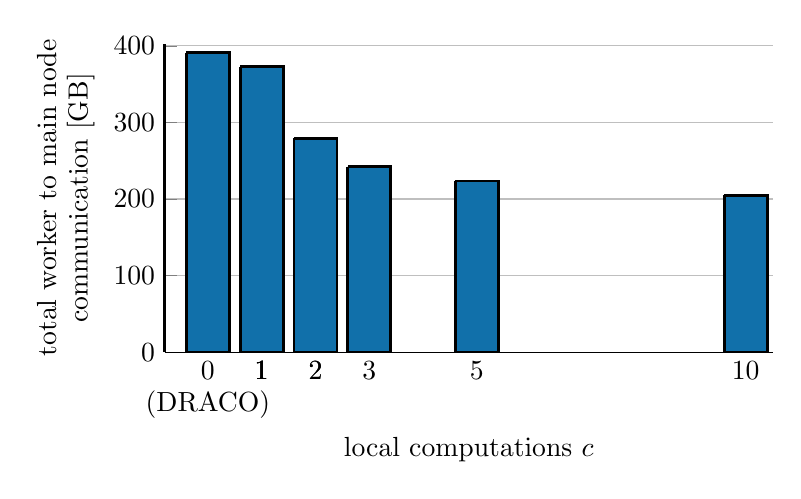
\begin{tikzpicture}
\begin{axis}[
legend cell align={left}, 
legend columns={1}, 
legend style={color={rgb,1:red,0.0;green,0.0;blue,0.0}, draw opacity={1.0}, line width={1}, solid, fill={rgb,1:red,1.0;green,1.0;blue,1.0}, fill opacity={1.0}, text opacity={1.0}, font={{\fontsize{8 pt}{10.4 pt}\selectfont}}, text={rgb,1:red,0.0;green,0.0;blue,0.0}, cells={anchor={center}}, at={(0.98, 0.98)}, anchor={north east}}, 
axis background/.style={fill={rgb,1:red,1.0;green,1.0;blue,1.0}, opacity={1.0}}, 
anchor={north west}, 
width={93mm}, 
height={55mm},
xlabel={local computations $c$}, 
x tick style={color={rgb,1:red,0.0;green,0.0;blue,0.0}, opacity={1.0}}, 
x tick label style={color={rgb,1:red,0.0;green,0.0;blue,0.0}, opacity={1.0}, rotate={0}}, 
xmin={-0.8}, 
xmax={10.5}, 
xtick={{10,5,3,2,2,1,1,1,1,1,0}}, 
xticklabels={{$10$,$5$,$3$,$2$,$2$,$1$,$1$,$1$,$1$,$1$,$0$\\(DRACO)}}, 
xtick align={inside}, 
xticklabel style={align=center},
axis x line*={left}, 
ylabel={total worker to main node\\communication [\si{\giga\byte}]}, 
ylabel style={align=center},
ymajorgrids={true}, 
ymin={0},
ymax={402.890145778656}, 
axis y line*={left}, 
y axis line style={color={rgb,1:red,0.0;green,0.0;blue,0.0}, draw opacity={1.0}, line width={1}, solid}, 
colorbar={false}]
    \addplot[color={rgb,1:red,0.0;green,0.0;blue,0.0}, name path={32f6c51a-9b4d-4fbc-8a2f-b9530c7ca1b0}, area legend, fill={rgb,1:red,0.0667;green,0.4392;blue,0.6667}, fill opacity={1.0}, draw opacity={1.0}, line width={1}, solid]
        table[row sep={\\}]
        {
            \\
            9.6  204.89096694160253  \\
            9.6  0.0  \\
            10.4  0.0  \\
            10.4  204.89096694160253  \\
            9.6  204.89096694160253  \\
        }
        ;
    \addplot[color={rgb,1:red,0.0;green,0.0;blue,0.0}, name path={32f6c51a-9b4d-4fbc-8a2f-b9530c7ca1b0}, area legend, fill={rgb,1:red,0.0667;green,0.4392;blue,0.6667}, fill opacity={1.0}, draw opacity={1.0}, line width={1}, solid, forget plot]
        table[row sep={\\}]
        {
            \\
            4.6  223.51741838199086  \\
            4.6  0.0  \\
            5.4  0.0  \\
            5.4  223.51741838199086  \\
            4.6  223.51741838199086  \\
        }
        ;
    \addplot[color={rgb,1:red,0.0;green,0.0;blue,0.0}, name path={32f6c51a-9b4d-4fbc-8a2f-b9530c7ca1b0}, area legend, fill={rgb,1:red,0.0667;green,0.4392;blue,0.6667}, fill opacity={1.0}, draw opacity={1.0}, line width={1}, solid, forget plot]
        table[row sep={\\}]
        {
            \\
            2.6  242.143869822224  \\
            2.6  0.0  \\
            3.4  0.0  \\
            3.4  242.143869822224  \\
            2.6  242.143869822224  \\
        }
        ;
    \addplot[color={rgb,1:red,0.0;green,0.0;blue,0.0}, name path={32f6c51a-9b4d-4fbc-8a2f-b9530c7ca1b0}, area legend, fill={rgb,1:red,0.0667;green,0.4392;blue,0.6667}, fill opacity={1.0}, draw opacity={1.0}, line width={1}, solid, forget plot]
        table[row sep={\\}]
        {
            \\
            1.6  260.7703212623019  \\
            1.6  0.0  \\
            2.4  0.0  \\
            2.4  260.7703212623019  \\
            1.6  260.7703212623019  \\
        }
        ;
    \addplot[color={rgb,1:red,0.0;green,0.0;blue,0.0}, name path={32f6c51a-9b4d-4fbc-8a2f-b9530c7ca1b0}, area legend, fill={rgb,1:red,0.0667;green,0.4392;blue,0.6667}, fill opacity={1.0}, draw opacity={1.0}, line width={1}, solid, forget plot]
        table[row sep={\\}]
        {
            \\
            1.6  279.39677270222455  \\
            1.6  0.0  \\
            2.4  0.0  \\
            2.4  279.39677270222455  \\
            1.6  279.39677270222455  \\
        }
        ;
    \addplot[color={rgb,1:red,0.0;green,0.0;blue,0.0}, name path={32f6c51a-9b4d-4fbc-8a2f-b9530c7ca1b0}, area legend, fill={rgb,1:red,0.0667;green,0.4392;blue,0.6667}, fill opacity={1.0}, draw opacity={1.0}, line width={1}, solid, forget plot]
        table[row sep={\\}]
        {
            \\
            0.6  298.023224141992  \\
            0.6  0.0  \\
            1.4  0.0  \\
            1.4  298.023224141992  \\
            0.6  298.023224141992  \\
        }
        ;
    \addplot[color={rgb,1:red,0.0;green,0.0;blue,0.0}, name path={32f6c51a-9b4d-4fbc-8a2f-b9530c7ca1b0}, area legend, fill={rgb,1:red,0.0667;green,0.4392;blue,0.6667}, fill opacity={1.0}, draw opacity={1.0}, line width={1}, solid, forget plot]
        table[row sep={\\}]
        {
            \\
            0.6  316.64967558160424  \\
            0.6  0.0  \\
            1.4  0.0  \\
            1.4  316.64967558160424  \\
            0.6  316.64967558160424  \\
        }
        ;
    \addplot[color={rgb,1:red,0.0;green,0.0;blue,0.0}, name path={32f6c51a-9b4d-4fbc-8a2f-b9530c7ca1b0}, area legend, fill={rgb,1:red,0.0667;green,0.4392;blue,0.6667}, fill opacity={1.0}, draw opacity={1.0}, line width={1}, solid, forget plot]
        table[row sep={\\}]
        {
            \\
            0.6  335.27612702106126  \\
            0.6  0.0  \\
            1.4  0.0  \\
            1.4  335.27612702106126  \\
            0.6  335.27612702106126  \\
        }
        ;
    \addplot[color={rgb,1:red,0.0;green,0.0;blue,0.0}, name path={32f6c51a-9b4d-4fbc-8a2f-b9530c7ca1b0}, area legend, fill={rgb,1:red,0.0667;green,0.4392;blue,0.6667}, fill opacity={1.0}, draw opacity={1.0}, line width={1}, solid, forget plot]
        table[row sep={\\}]
        {
            \\
            0.6  353.90257846036303  \\
            0.6  0.0  \\
            1.4  0.0  \\
            1.4  353.90257846036303  \\
            0.6  353.90257846036303  \\
        }
        ;
    \addplot[color={rgb,1:red,0.0;green,0.0;blue,0.0}, name path={32f6c51a-9b4d-4fbc-8a2f-b9530c7ca1b0}, area legend, fill={rgb,1:red,0.0667;green,0.4392;blue,0.6667}, fill opacity={1.0}, draw opacity={1.0}, line width={1}, solid, forget plot]
        table[row sep={\\}]
        {
            \\
            0.6  372.5290298995096  \\
            0.6  0.0  \\
            1.4  0.0  \\
            1.4  372.5290298995096  \\
            0.6  372.5290298995096  \\
        }
        ;
    \addplot[color={rgb,1:red,0.0;green,0.0;blue,0.0}, name path={32f6c51a-9b4d-4fbc-8a2f-b9530c7ca1b0}, area legend, fill={rgb,1:red,0.0667;green,0.4392;blue,0.6667}, fill opacity={1.0}, draw opacity={1.0}, line width={1}, solid, forget plot]
        table[row sep={\\}]
        {
            \\
            -0.4  391.155481338501  \\
            -0.4  0.0  \\
            0.4  0.0  \\
            0.4  391.155481338501  \\
            -0.4  391.155481338501  \\
        }
        ;
    \addplot[color={rgb,1:red,0.0667;green,0.4392;blue,0.6667}, name path={9bed8f1c-8a16-44ab-bc3c-0b56859e86c4}, only marks, draw opacity={1.0}, line width={0}, solid, mark={*}, mark size={0.0 pt}, mark repeat={1}, mark options={color={rgb,1:red,0.0;green,0.0;blue,0.0}, draw opacity={0.0}, fill={rgb,1:red,0.0667;green,0.4392;blue,0.6667}, fill opacity={0.0}, line width={0.75}, rotate={0}, solid}, forget plot]
        table[row sep={\\}]
        {
            \\
            10.0  204.89096694160253  \\
            5.0  223.51741838199086  \\
            3.0  242.143869822224  \\
            2.0  260.7703212623019  \\
            2.0  279.39677270222455  \\
            1.0  298.023224141992  \\
            1.0  316.64967558160424  \\
            1.0  335.27612702106126  \\
            1.0  353.90257846036303  \\
            1.0  372.5290298995096  \\
            0.0  391.155481338501  \\
        }
        ;
\end{axis}
\end{tikzpicture}

    }
    \vspace{-1.1em}
    \caption{Tradeoff between total worker to main-node communication and number of local computations for our scheme. The parameters are $\nmalicious = 10$, $1 \leq \nhonest \leq 11$, $\ngroup=1$, $\ngrad = \num{1e4}$, $\graddim=\num{1e6}$, $|\galpha|=2^{16}$. When considering total communication, the cost of the protocol is outweighed by the cost of transmitting the gradient values. The gap to our bound, given in \cref{thm:converse_T}, is less than \SI{5}{\kilo\byte}.
    For $\localcomp=0$ local computations, our scheme is equivalent to DRACO~\cite{chenDRACOByzantineresilientDistributed2018}.
    By requiring less workers, our scheme with $\nhonest=1$ reduces communication by \SI{48}{\percent} at the expense of at most $\localcomp=10$ local gradient computations at the \master. For comparison, each worker node performs $\ngrad=\num{1e4}$ gradient computations.}
    \label{fig:comm_vs_localcomp}
    \vspace{-1.4em}
\end{figure}

As depicted in \cref{fig:comm_vs_localcomp}, for realistic parameter ranges, the local computations drastically reduce the required communication. The communication overhead of the protocol $\commoh$ is outweighed by the initial transmission of $\iresp_{0, \wind}$. For a comparison between our achievability result and converse for $\commoh$, cf. \cref{app:achievability_vs_converse}. 

We prove our lower bounds by considering the case where the adversary chooses the following behaviour for the malicious workers.

\subsection{Symmetrization Attack for Bounds}\label{sec:attack}
    The adversary chooses a (potentially corrupted) value for each malicious worker and each partial gradient. 
    We denote worker $\worker$'s \emph{claimed} partial gradient results for $\pgrad$ as $\wpgrad{\gind}{\wind}\in\galpha^\graddim$ for all $\wind \in \range{\nworker}$ and $\gind\in\range{\ngrad}$.
    For honest workers we say $\wpgrad{\gind}{\wind} = \pgrad[\gind]$.
    Each worker $\worker$ computes their responses consistently based on those values, i.e.,
    \begin{align*}
        \noisyiresp_{\roundind, \wind} &= \encfun[\wind,\encind_{\wind,\roundind}]\left( \wpgrad{1}{\wind},\dots,\wpgrad{\ngrad}{\wind} \right),\\ 
        &\forall \roundind\in \{0, \dots, \nround\}, \wind \in \range{\nworker}, \encind_\wind \in \range{\nencfun}.
    \end{align*}
    For clarity of exposition, we first lay out how the adversary chooses the claimed gradient values for $\ngroup=1$ groups of size $\nmalicious+1$, i.e., $\nhonest=1$, before we generalize to arbitrary $\ngroup, \nhonest \in \N$.

    For $\nhonest=1$ and $\ngroup=1$, the adversary draws a set $\disagreegradset \subseteq \range{\ngrad}$ of size $|\disagreegradset|=\lfloor \frac{\nmalicious}{\nhonest} \rfloor = \nmalicious$ uniformly at random and assigns each malicious worker $\worker$ a unique gradient index from $\disagreegradset$.
    For each index, it sets the corresponding worker's claimed value to a distinct random vector unequal the true value and all other malicious worker's values to the true partial gradient value.
    With probability $\frac{1}{2}$, it picks a single gradient index from $\disagreegradset$ uniformly at random and sets all malicious workers' values to the same erroneous random partial gradient value.
    The resulting claimed gradients take on the form as depicted in \cref{tab:key_error_pattern}.
\begin{table}[h]
    \vspace{-0.3cm}
    \begin{tabularx}{\columnwidth}{c|ccccccc}
        & $\wpgrad{1}{\wind}$ & $\wpgrad{2}{\wind}$ 
        & $\dots$  & $\wpgrad{\nmalicious}{\wind}$ & $\wpgrad{\nmalicious+1}{\wind}$ & $\dots$ & $\wpgrad{\ngrad}{\wind}$ \\ 
        \toprule
        $\worker[1]$ & $\pgrad[1]^{\prime\prime}$ & $\pgrad[2]^\prime$ & $\dots$  & $\pgrad[\nmalicious]^\prime$ & $\pgrad[\nmalicious+1]^\prime$ & $\dots$ & $\pgrad[\ngrad]^\prime$ \\ 
        $\worker[2]$ & $\pgrad[1]^\prime$ & $\pgrad[2]^{\prime\prime}$ & $\dots$  & $\pgrad[\nmalicious]^\prime$ & $\pgrad[\nmalicious+1]^\prime$ & $\dots$ & $\pgrad[\ngrad]^\prime$ \\ 
        $\vdots$ & $\vdots$ & $\vdots$ & $\ddots$ & $\vdots$ & $\vdots$ & $\dots$ & $\vdots$ \\
        $\worker[\nmalicious]$ & $\pgrad[1]^\prime$ & $\pgrad[2]^\prime$ & $\dots$ & $\pgrad[\nmalicious]^{\prime\prime}$ & $\pgrad[\nmalicious+1]^\prime$ & $\dots$ & $\pgrad[\ngrad]^\prime$ \\ 
       $\worker[\nmalicious+1]$ & $\pgrad[1]^\prime$ & $\pgrad[2]^\prime$ & $\dots$  & $\pgrad[\nmalicious]^\prime$ & $\pgrad[\nmalicious + 1]^\prime$ & $\dots$ & $\pgrad[\ngrad]^\prime$ \\ 
    \end{tabularx}
    \caption{claimed partial gradients for symmetrization attack.}
    \vspace{-0.5cm}
    \label{tab:key_error_pattern}
\end{table}
    For partial gradients with index in $\disagreegradset$ there are two competing values $\pgrad^{\prime}$ and $\pgrad^{\prime\prime}$ whereas for all other gradient indices the claimed values by all workers agree.

    For $\nhonest > 1$, the adversary randomly partitions the malicious workers into $\lfloor \nmalicious / \nhonest \rfloor -1$ sets of size $\nhonest$ and (depending on divisibility) one group of size $\nmalicious \mod \nhonest$.
    Each of the sets of size $\nhonest$ behaves like one malicious worker in the case $\nhonest=1$.
    The workers in the remaining set of less than $\nhonest$ workers (if non-empty) pick their claimed gradients randomly either like a random other set of workers or like the honest workers.
    The resulting claimed gradients take on the form as depicted in \cref{tab:key_error_pattern_generalized} in Appendix~\ref{app:large_table}.

For $\ngroup > 1$, the adversary chooses the first group and chooses the claimed gradients according to the attack strategy for $\ngroup^\prime=1$ and $\ngrad^\prime=\ngrad / \ngroup$ in that group. In all other groups, the claimed gradients are equal to their true values.

\subsection{Fundamental Limits}

\begin{theorem}[Lower bound on $\localcomp$ and $\replfact$]
Suppose that $\nworker = \ngroup (\nmalicious + \nhonest)$ for integers $\ngroup,\nhonest \geq 1$. For any tuple (\allocmat, \encfunset, \decfun, \proto), with $\allocmat$ as in \eqref{eq:fractional_repetition}, to be a (\nround,\localcomp,\replfact,\commoh)-\BGC scheme, it holds that if $\replfact \leq \nmalicious + \nhonest$, then $\localcomp\geq \compbound$ (conversely,  if $\localcomp < \compbound$ then $\replfact > {\nmalicious + \nhonest}$) for any number of rounds $\nround$ and any communication overhead $\commoh$. 
\label{thm:converse_C}
\end{theorem}
\begin{IEEEproof}
    We demonstrate that any tuple $(\allocmat, \encfunset, \decfun, \proto)$ with fractional repetition data allocation which uses $\localcomp \leq \compbound - 1$ local computations cannot be an \BGC scheme. Specifically, we show that the malicious workers can always perform a symmetrization attack preventing the main node from deterministically computing the full gradient. 
    Let the malicious workers behave as explained in \cref{sec:attack}. 

    We abstract $\encfunset$ and $\proto_1$ by assuming that the values of all partial gradients $\wpgrad{\gind}{\wind}$ computed by the workers are available at the \master. Note that regardless of $\encfunset$ and $\proto_1$ the \master cannot gain any additional information from the workers' responses.
    We now show that for $\localcomp \leq \compbound-1$ there exists no choice of a decoding function $\decfun$ and $\proto_2$ for which the \master deterministically outputs the true full gradient. To that end, for any possible $\proto_2$, we give two cases for which the inputs to the decoding function are identical but the true full gradients differ.

    The claimed partial gradients take on values as in \cref{tab:key_error_pattern} for $\nhonest=1$ and \cref{tab:key_error_pattern_generalized} for $\nhonest>1$. There are $\compbound$ partial gradients, say $\pgrad[1],\ldots,\pgrad[\compbound]$, such that for each partial gradient $\pgrad[\gind]$ worker $\worker[\gind]$ sends a value $\wpgrad{\gind}{\gind} = \pgrad[\gind]^{\prime\prime}$ that is different from the value $\pgrad[i]^\prime$ sent by all other workers.
For any list $\lgindset^{(\nround)}$ of locally computed gradients of size $|\lgindset^{(\nround)}| \leq \nmalicious-1$ (produced by any $\proto_2$) there exists an index $\widetilde{\gind} \in [\nmalicious]$ such that $\widetilde{\gind} \notin \lgindset^{(\nround)}$.
Consider the following two cases:\begin{enumerate}[label=Case \arabic{*}:, wide=1.5\parindent, leftmargin=*]
    \item $\pgrad[\gind] = \pgrad[\gind]^\prime \;\forall \gind \in [\frac{\ngrad}{\ngroup}]$ and 
    \item $\pgrad[\gind] = \pgrad[\gind]^\prime \;\forall \gind \in [\frac{\ngrad}{\ngroup}] \setminus \{\widetilde{\gind}\}$ and $\pgrad[\widetilde{\gind}] = \pgrad[\widetilde{\gind}]^{\prime\prime}$.
\end{enumerate}
It is easy to see that both cases occur with non-zero probability according to the attack strategy in \cref{sec:attack}. In both cases, the inputs to $\decfun$ only depend on the fixed $\lgindset^{(\nround)}$, the $\wpgrad{\gind}{\wind},\;\wind \in [\nmalicious +1],\;\gind\in[\frac{\ngrad}{\ngroup}]$ and the $\pgrad[\gind],\; \gind \in \lgindset^{(\nround)}$, all of which take on identical values in both cases.
The value of the full gradient $\tgrad$, however, is $\sum_{\gind \in [\ngrad]} \pgrad[\gind]^\prime$ in Case 1 and $\pgrad[\widetilde{\gind}]^{\prime\prime} + \sum_{\gind \in [\ngrad] \setminus \{\widetilde{\gind}\}} \pgrad[\gind]^\prime$ in Case 2. Hence, for $\localcomp < \compbound$ no decoding function can deterministically produce the correct full gradient.
\end{IEEEproof}

\begin{theorem}[Lower bound on $\commoh$ for fixed $\localcomp$ and $\replfact$]
Suppose that $\nworker = \ngroup (\nmalicious + \nhonest)$ for integers $\ngroup,\nhonest \geq 1$. For any tuple (\allocmat, \encfunset, \decfun, \proto), with $\allocmat$ as in \eqref{eq:fractional_repetition}, to be a (\nround,\localcomp,\replfact,\commoh)-\BGC scheme with $\replfact = {\nmalicious + \nhonest}$ and $\localcomp = \compbound$, then it must hold that
  \vspace{-0.6em}
    \begin{align*}
        \commoh \geq {\log_{\alphasize} \binom{\ngrad/\ngroup}{\lfloor \nmalicious / \nhonest \rfloor}}.%
    \end{align*}
  \vspace{-0.6em}
    \label{thm:converse_T}
\end{theorem}

\vspace{-0.3cm}
\begin{IEEEproof}
The proof is given in \cref{sec:proof_lower_bound_kappa_rho}
\end{IEEEproof}

\subsection{Construction of an \BGC Scheme}

\begin{theorem}
  The scheme constructed below is an \BGC scheme with a parameter $\nhonest$ such that $1\leq \nhonest \leq \nmalicious+1$ and requires $\nround \leq \left(\nmalicious+1-\nhonest\right) \left\lceil \log_2\left(\frac{\ngrad}{\ngroup}\right) \right\rceil$ rounds, $\localcomp \leq \compbound$ local gradient computations, $\replfact = {\nmalicious+\nhonest}$, and $\commoh \leq \left(\nmalicious+1-\nhonest\right) \left( 2 \left\lceil \log_2\left( \frac{\ngrad}{\ngroup}\right) \right\rceil+ \frac{\nmalicious+3\nhonest}{2\log_2{\card{\galpha}}} \right)$. 
    \label{thm:scheme}
\end{theorem}
\begin{IEEEproof}
    We defer the proof to Appendix~\ref{app:scheme_proof}.
\end{IEEEproof}

We construct an $(\nround, \localcomp, \replfact, \commoh)$-\BGC scheme that has a replication factor $\replfact={\nmalicious+\nhonest}$, $\nhonest \geq 1$, and requires the optimal local computation load $\localcomp \leq \compbound$ at the \master. The protocol $\proto$ runs for $\nround \leq \left(\nmalicious+1-\nhonest\right) \left\lceil \log_2\left(\frac{\ngrad}{\ngroup}\right) \right\rceil$ rounds and achieves a communication overhead \mbox{$\commoh \leq \left(\nmalicious+1-\nhonest\right) \left( 2 \left\lceil \log_2\left( \frac{\ngrad}{\ngroup}\right) \right\rceil+ \frac{\nmalicious+3\nhonest}{2\log_2{\card{\galpha}}} \right)$}. Our scheme uses a fractional repetition data assignment with $\ngroup$ groups each of size $\nmalicious+\nhonest$. Informally, in each group, the \master runs an elimination tournament consisting of matches (similar to the one explained in~\cref{ex:toy_problem}) between pairs of workers that return contradicting responses. An algorithmic description of the elimination tournament is given in \cref{alg:elimination_tournament} for the general case. For clarity of exposition, we explain the idea of our scheme for the special case of $\nhonest=1$. The general case for $\nhonest\geq 2$ follows similar steps and is given in \cref{app:general_case}.

The tournament consists of a series of matches between two workers. 
During a match, each worker constructs a binary tree based on their computed partial gradients, which we refer to as the match tree.
The root of the tree is labeled by the sum of all partial gradients computed at that worker ($\noisyiresp_{0,\wind}$).
The child nodes are constructed based on the partial gradients that are contained in the parent node.
Each node has two children: the first one is labeled by the sum of the first half of the parent node's partial gradients; the second one is labeled by the sum of the second half of the parent node's partial gradients.
Thus, the labeling is done such that the sum of the labels of any two siblings gives the label of their parent node.

Proceeding in this way recursively, each worker ends up with the leaves of the tree being labeled by individual partial gradients.
For example, when $\ngroup = 1$ and $\ngrad=4$, the tree is depicted in \cref{fig:binary_add_tree}.
During a match, the \master requests the labels for particular nodes in this tree from the two competing workers, and compares them. 
If the root labels of two match trees differ, then by definition there must be a child node for which the corresponding label differs in those trees. By induction, it is clear that there has to be a path from the root to a leaf, such that the corresponding labels of all involved nodes differ between the two match trees. Applying this observation to the example in \cref{fig:binary_add_tree}, if $\wpgrad{1}{\wind}+\wpgrad{2}{\wind}+\wpgrad{3}{\wind}+\wpgrad{4}{\wind}$ is different for two workers, then $\wpgrad{1}{\wind}+\wpgrad{2}{\wind}$ or $\wpgrad{3}{\wind}+\wpgrad{4}{\wind}$ must also differ (or both). In the latter case, we end up with $\wpgrad{3}{\wind}$ or $\wpgrad{4}{\wind}$ being different between the workers.
\begin{figure}[h]
  \vspace{-0.8em}
    \centering
    \resizebox{0.9\linewidth}{!}{
    \begin{tikzpicture}
\def\angle{45}
\node {$\wpgrad{1}{\wind}+\wpgrad{2}{\wind}+\wpgrad{3}{\wind}+\wpgrad{4}{\wind}$} [sibling distance = 5cm,level distance=0.8cm]
    child {node (a) {$\wpgrad{1}{\wind}+\wpgrad{2}{\wind}$} [sibling distance = 2.5cm,level distance=1cm]
        child {node {$\wpgrad{1}{\wind}$}}
        child {node (y) {$\wpgrad{2}{\wind}$}}
    } 
    child {node (d) {$\wpgrad{3}{\wind}+\wpgrad{4}{\wind}$} [sibling distance = 2.5cm,level distance=0.8cm]
        child {node (z) {$\wpgrad{3}{\wind}$}}
        child {node {$\wpgrad{4}{\wind}$}}
    };
\end{tikzpicture}

    }
  \vspace{-1em}
    \caption{Example of a match tree for $\worker$ and parameters $\ngroup=1,\ngrad=4$.}
    \label{fig:binary_add_tree}
\end{figure}

The match starts at the root. In this case, each worker $\worker$ would have already sent the node label in $\iresp_{0,\wind}$ to the \master, i.e.,
  \vspace{-0.6em}
\begin{equation*}
    \iresp_{0,\wind} = \encfun[\wind,1]\left( \pgrad[1],\dots,\pgrad[\ngrad] \right) = \sum_{\substack{ \gind \in \range{\ngrad} \\ \allocmat[\gind, \wind] = 1}} \pgrad[\gind].
  \vspace{-0.8em}
\end{equation*}
Note that, without errors, all workers' messages agree within a group.
In case of discrepancies between the responses $\noisyiresp_{0,\wind}$ of the workers within a group, the \master selects a pair of disagreeing workers $\worker[\wind_1],\worker[\wind_2]$ and further descends in the tree as follows.

For every node in the tree, the \master requests and compares the left child's label from both workers, encoded in $\iresp_{\roundind,\indone}$ and $\iresp_{\roundind,\indtwo}$. The \master then moves on to a child whose label the workers disagree on.
Note that, based on the current node's label and the left child's label, the \master can infer the right child's label.
If the competing workers agree on the left child's label, they must disagree on the right child's label.
This procedure is repeated until a leaf is reached.
Note that, even if the workers send inconsistent labels at each round, this procedure is guaranteed to reach a leaf node for which the (sent or inferred) values of the individual gradient is different for the two workers. \cref{alg:match} formalizes this procedure for $\ngroup=1$.

Note that it is possible to reduce the communication load by picking a coordinate $\compind$ in which the workers' initial responses disagree, i.e., $\comp{ \iresp_{0,\indone} } \neq \comp{ \iresp_{0,\indtwo} }$. That is, the workers only encode the $\compind$-th coordinate of the node labels. By this method, it is still guaranteed that the \master can identify a partial gradient for which the competing workers disagree.

Having identified disagreeing values $\wpgrad{\gind}{\wind_1}$ and $\wpgrad{\gind}{\wind_2}$ of a partial gradient $\pgrad[\gind]$, the \master computes the correct of this partial gradient locally. It then marks the worker(s) whose values differ from the value computed locally as malicious.
The algorithm ends up with disagreeing leaf labels by design. Therefore, each match is guaranteed to eliminate at least one malicious worker and no honest workers.
After performing at most $\nmalicious$ matches, the \master is guaranteed to identify all malicious workers.
The \master takes the encoded gradient of one worker identified as being honest from each group and sums up the group-wise results to obtain $\gestim=\tgrad$.

\subsection{Discussion}
According to \cref{thm:converse_C}, the interactive protocol of our scheme achieves the lowest possible number of locally computed partial gradients for the fractional repetition data assignment and $\replfact = \nmalicious+\nhonest$. Note that for $\nhonest \geq \nmalicious+1$, i.e., $\replfact \geq 2\nmalicious+1$, no local computation is necessary. In fact, since there is only one set of consistent workers $\workerset$ that has $\card{\workerset} \geq \nhonest$ per fractional repetition group, the scheme immediately identifies $\workerset$ as the honest set and terminates without any additional computation or communication. Thus, as shown in~\cite{chenDRACOByzantineresilientDistributed2018}, our scheme achieves the optimal performance in this case. Although we consider $1 \leq \nhonest \leq \nmalicious+1$ in \cref{thm:scheme} for technical reasons, the scheme works for any $\nhonest \geq 1$.
Note that the achievable bound on $\commoh$ in \cref{thm:scheme} is off from the converse bound in \cref{thm:converse_T} by a constant factor asymptotically, see \cref{fig:achievability_vs_converse_datacolumns} in Appendix~\ref{app:achievability_vs_converse}. The reason is that we use a rather simple and conservative lower bound on the amount of information that is required to be transmitted by the workers in \cref{thm:converse_T}. Among others, we assume that all workers have knowledge about the malicious worker's identities and also the malicious workers contribute useful information. Improvement of the converse bound is left for future work.

\section{Conclusion}\label{sec:conclusion}
In this work, we focus on addressing the fundamental challenge of OOD detection tasks, which is how to fully understand the semantic discrepancy between the ID/OOD samples. We reveal that the key to success in the realistic SCOOD task is to allocate as many ID samples in the unlabeled set correctly as possible. To this end, we propose a novel uncertainty-aware optimal transport scheme that introduces class-specific energy scores as guidance for effective label assignment. Experimental results show that our method achieves better performance than previous state-of-the-art methods on SCOOD benchmarks.

\textbf{Limitations.} In addition to temperature scaling, other techniques such as feature clipping applied in ReAct~\cite{sun2021react} also enhance the performance of energy score, so how to obtain an OOD score that best fits the SCOOD task can be further explored. Moreover, a setting highly related to SCOOD has been proposed in \cite{katz2022training} and formulated as a constrained optimization problem. We will also theoretically analyze these practical OOD settings in our feature work.

% \section*{Acknowledgments}
\textbf{Acknowledgments.} 
This work is supported by National Key R\&D Program of China under Grant 2020AAA0105701, National Natural Science Foundation of China (NSFC) under Grants 61872327, Major Special Science and Technology Project of Anhui, National Natural Science Foundation of China (62033012) and Ant Group through Ant Research Intern Program.


\balance
\bibliographystyle{IEEEtran}
%%% -*-BibTeX-*-
%%% Do NOT edit. File created by BibTeX with style
%%% ACM-Reference-Format-Journals [18-Jan-2012].

\begin{thebibliography}{52}

%%% ====================================================================
%%% NOTE TO THE USER: you can override these defaults by providing
%%% customized versions of any of these macros before the \bibliography
%%% command.  Each of them MUST provide its own final punctuation,
%%% except for \shownote{}, \showDOI{}, and \showURL{}.  The latter two
%%% do not use final punctuation, in order to avoid confusing it with
%%% the Web address.
%%%
%%% To suppress output of a particular field, define its macro to expand
%%% to an empty string, or better, \unskip, like this:
%%%
%%% \newcommand{\showDOI}[1]{\unskip}   % LaTeX syntax
%%%
%%% \def \showDOI #1{\unskip}           % plain TeX syntax
%%%
%%% ====================================================================

\ifx \showCODEN    \undefined \def \showCODEN     #1{\unskip}     \fi
\ifx \showDOI      \undefined \def \showDOI       #1{#1}\fi
\ifx \showISBNx    \undefined \def \showISBNx     #1{\unskip}     \fi
\ifx \showISBNxiii \undefined \def \showISBNxiii  #1{\unskip}     \fi
\ifx \showISSN     \undefined \def \showISSN      #1{\unskip}     \fi
\ifx \showLCCN     \undefined \def \showLCCN      #1{\unskip}     \fi
\ifx \shownote     \undefined \def \shownote      #1{#1}          \fi
\ifx \showarticletitle \undefined \def \showarticletitle #1{#1}   \fi
\ifx \showURL      \undefined \def \showURL       {\relax}        \fi
% The following commands are used for tagged output and should be
% invisible to TeX
\providecommand\bibfield[2]{#2}
\providecommand\bibinfo[2]{#2}
\providecommand\natexlab[1]{#1}
\providecommand\showeprint[2][]{arXiv:#2}

\bibitem[\protect\citeauthoryear{Albrecht and Stone}{Albrecht and
  Stone}{2017}]%
        {Albrecht2017ReasoningAH}
\bibfield{author}{\bibinfo{person}{Stefano~V. Albrecht} {and}
  \bibinfo{person}{P. Stone}.} \bibinfo{year}{2017}\natexlab{}.
\newblock \showarticletitle{Reasoning about Hypothetical Agent Behaviours and
  their Parameters}. In \bibinfo{booktitle}{\emph{AAMAS}}.
\newblock


\bibitem[\protect\citeauthoryear{Andrejczuk, Berger, Rodriguez-Aguilar, Sierra,
  and Mar{\'\i}n-Puchades}{Andrejczuk et~al\mbox{.}}{2018}]%
        {andrejczuk2018composition}
\bibfield{author}{\bibinfo{person}{Ewa Andrejczuk}, \bibinfo{person}{Rita
  Berger}, \bibinfo{person}{Juan~A Rodriguez-Aguilar}, \bibinfo{person}{Carles
  Sierra}, {and} \bibinfo{person}{V{\'\i}ctor Mar{\'\i}n-Puchades}.}
  \bibinfo{year}{2018}\natexlab{}.
\newblock \showarticletitle{The composition and formation of effective teams:
  computer science meets organizational psychology}.
\newblock \bibinfo{journal}{\emph{The Knowledge Engineering Review}}
  \bibinfo{volume}{33} (\bibinfo{year}{2018}), \bibinfo{pages}{e17}.
\newblock


\bibitem[\protect\citeauthoryear{Arjona-Medina, Gillhofer, Widrich,
  Unterthiner, Brandstetter, and Hochreiter}{Arjona-Medina
  et~al\mbox{.}}{2019}]%
        {arjona2019rudder}
\bibfield{author}{\bibinfo{person}{Jose~A Arjona-Medina},
  \bibinfo{person}{Michael Gillhofer}, \bibinfo{person}{Michael Widrich},
  \bibinfo{person}{Thomas Unterthiner}, \bibinfo{person}{Johannes
  Brandstetter}, {and} \bibinfo{person}{Sepp Hochreiter}.}
  \bibinfo{year}{2019}\natexlab{}.
\newblock \showarticletitle{Rudder: Return decomposition for delayed rewards}.
\newblock \bibinfo{journal}{\emph{NeurIPS}}  \bibinfo{volume}{32}
  (\bibinfo{year}{2019}).
\newblock


\bibitem[\protect\citeauthoryear{Beal, Changder, Norman, and Ramchurn}{Beal
  et~al\mbox{.}}{2020}]%
        {beal2020learning}
\bibfield{author}{\bibinfo{person}{Ryan Beal}, \bibinfo{person}{Narayan
  Changder}, \bibinfo{person}{Timothy Norman}, {and} \bibinfo{person}{Sarvapali
  Ramchurn}.} \bibinfo{year}{2020}\natexlab{}.
\newblock \showarticletitle{Learning the value of teamwork to form efficient
  teams}. In \bibinfo{booktitle}{\emph{Proceedings of the AAAI Conference on
  Artificial Intelligence}}, Vol.~\bibinfo{volume}{34}.
  \bibinfo{pages}{7063--7070}.
\newblock


\bibitem[\protect\citeauthoryear{Beetz, Hoyningen-Huene, Bandouch,
  Kirchlechner, Gedikli, and Maldonado}{Beetz et~al\mbox{.}}{2006}]%
        {beetz2006camera}
\bibfield{author}{\bibinfo{person}{Michael Beetz}, \bibinfo{person}{Nico~v
  Hoyningen-Huene}, \bibinfo{person}{Jan Bandouch}, \bibinfo{person}{Bernhard
  Kirchlechner}, \bibinfo{person}{Suat Gedikli}, {and} \bibinfo{person}{Alexis
  Maldonado}.} \bibinfo{year}{2006}\natexlab{}.
\newblock \showarticletitle{Camera-based observation of football games for
  analyzing multi-agent activities}. In \bibinfo{booktitle}{\emph{Proceedings
  of the fifth international joint conference on Autonomous agents and
  multiagent systems}}. \bibinfo{pages}{42--49}.
\newblock


\bibitem[\protect\citeauthoryear{Bialkowski, Lucey, Carr, Yue, Sridharan, and
  Matthews}{Bialkowski et~al\mbox{.}}{2014}]%
        {bialkowski2014large}
\bibfield{author}{\bibinfo{person}{Alina Bialkowski}, \bibinfo{person}{Patrick
  Lucey}, \bibinfo{person}{Peter Carr}, \bibinfo{person}{Yisong Yue},
  \bibinfo{person}{Sridha Sridharan}, {and} \bibinfo{person}{Iain Matthews}.}
  \bibinfo{year}{2014}\natexlab{}.
\newblock \showarticletitle{Large-scale analysis of soccer matches using
  spatiotemporal tracking data}. In \bibinfo{booktitle}{\emph{2014 IEEE
  international conference on data mining}}. IEEE, \bibinfo{pages}{725--730}.
\newblock


\bibitem[\protect\citeauthoryear{Bouveret and Lang}{Bouveret and Lang}{2014}]%
        {bouveret2014manipulating}
\bibfield{author}{\bibinfo{person}{Sylvain Bouveret} {and}
  \bibinfo{person}{J{\'e}r{\^o}me Lang}.} \bibinfo{year}{2014}\natexlab{}.
\newblock \showarticletitle{Manipulating picking sequences.}. In
  \bibinfo{booktitle}{\emph{ECAI}}, Vol.~\bibinfo{volume}{14}.
  \bibinfo{pages}{141--146}.
\newblock


\bibitem[\protect\citeauthoryear{Brams and Straffin~Jr}{Brams and
  Straffin~Jr}{1979}]%
        {brams1979prisoners}
\bibfield{author}{\bibinfo{person}{Steven~J Brams} {and}
  \bibinfo{person}{Philip~D Straffin~Jr}.} \bibinfo{year}{1979}\natexlab{}.
\newblock \showarticletitle{Prisoners' dilemma and professional sports drafts}.
\newblock \bibinfo{journal}{\emph{The American Mathematical Monthly}}
  \bibinfo{volume}{86}, \bibinfo{number}{2} (\bibinfo{year}{1979}),
  \bibinfo{pages}{80--88}.
\newblock


\bibitem[\protect\citeauthoryear{Bransen and Van~Haaren}{Bransen and
  Van~Haaren}{2020}]%
        {bransen2020player}
\bibfield{author}{\bibinfo{person}{Lotte Bransen} {and} \bibinfo{person}{Jan
  Van~Haaren}.} \bibinfo{year}{2020}\natexlab{}.
\newblock \showarticletitle{Player chemistry: Striving for a perfectly balanced
  soccer team}.
\newblock \bibinfo{journal}{\emph{Sports Analytics Conference}}
  (\bibinfo{year}{2020}).
\newblock


\bibitem[\protect\citeauthoryear{Dafoe, Bachrach, Hadfield, Horvitz, Larson,
  and Graepel}{Dafoe et~al\mbox{.}}{2021}]%
        {DafoeNature2021}
\bibfield{author}{\bibinfo{person}{Allan Dafoe}, \bibinfo{person}{Yoram
  Bachrach}, \bibinfo{person}{Gillian Hadfield}, \bibinfo{person}{Eric
  Horvitz}, \bibinfo{person}{Kate Larson}, {and} \bibinfo{person}{Thore
  Graepel}.} \bibinfo{year}{2021}\natexlab{}.
\newblock \showarticletitle{Cooperative {AI}: machines must learn to find
  common ground}.
\newblock \bibinfo{journal}{\emph{Nature}}  \bibinfo{volume}{593}
  (\bibinfo{year}{2021}), \bibinfo{pages}{33--36}.
\newblock


\bibitem[\protect\citeauthoryear{Derks and Peters}{Derks and Peters}{1993}]%
        {derks1993shapley}
\bibfield{author}{\bibinfo{person}{Jean Derks} {and} \bibinfo{person}{Hans
  Peters}.} \bibinfo{year}{1993}\natexlab{}.
\newblock \showarticletitle{A Shapley value for games with restricted
  coalitions}.
\newblock \bibinfo{journal}{\emph{International Journal of Game Theory}}
  \bibinfo{volume}{21}, \bibinfo{number}{4} (\bibinfo{year}{1993}),
  \bibinfo{pages}{351--360}.
\newblock


\bibitem[\protect\citeauthoryear{Durugkar, Liebman, and Stone}{Durugkar
  et~al\mbox{.}}{2020}]%
        {Durugkar2020BalancingIP}
\bibfield{author}{\bibinfo{person}{Ishan Durugkar}, \bibinfo{person}{E.
  Liebman}, {and} \bibinfo{person}{P. Stone}.} \bibinfo{year}{2020}\natexlab{}.
\newblock \showarticletitle{Balancing Individual Preferences and Shared
  Objectives in Multiagent Reinforcement Learning}. In
  \bibinfo{booktitle}{\emph{IJCAI}}.
\newblock


\bibitem[\protect\citeauthoryear{Elitzur}{Elitzur}{2020}]%
        {elitzur2020data}
\bibfield{author}{\bibinfo{person}{Ramy Elitzur}.}
  \bibinfo{year}{2020}\natexlab{}.
\newblock \showarticletitle{Data analytics effects in major league baseball}.
\newblock \bibinfo{journal}{\emph{Omega}}  \bibinfo{volume}{90}
  (\bibinfo{year}{2020}), \bibinfo{pages}{102001}.
\newblock


\bibitem[\protect\citeauthoryear{Ellis}{Ellis}{1983}]%
        {ellis1983similarities}
\bibfield{author}{\bibinfo{person}{M Ellis}.} \bibinfo{year}{1983}\natexlab{}.
\newblock \showarticletitle{Similarities and differences in games: A system for
  classification}. In \bibinfo{booktitle}{\emph{International association for
  physical education in higher education Conference}}.
\newblock


\bibitem[\protect\citeauthoryear{Fern{\'a}ndez, Bornn, and
  Cervone}{Fern{\'a}ndez et~al\mbox{.}}{2021}]%
        {fernandez2021framework}
\bibfield{author}{\bibinfo{person}{Javier Fern{\'a}ndez}, \bibinfo{person}{Luke
  Bornn}, {and} \bibinfo{person}{Daniel Cervone}.}
  \bibinfo{year}{2021}\natexlab{}.
\newblock \showarticletitle{A framework for the fine-grained evaluation of the
  instantaneous expected value of soccer possessions}.
\newblock \bibinfo{journal}{\emph{Machine Learning}} \bibinfo{volume}{110},
  \bibinfo{number}{6} (\bibinfo{year}{2021}), \bibinfo{pages}{1389--1427}.
\newblock


\bibitem[\protect\citeauthoryear{Fisac, Bronstein, Stefansson, Sadigh, Sastry,
  and Dragan}{Fisac et~al\mbox{.}}{2019}]%
        {fisac2019hierarchical}
\bibfield{author}{\bibinfo{person}{Jaime~F Fisac}, \bibinfo{person}{Eli
  Bronstein}, \bibinfo{person}{Elis Stefansson}, \bibinfo{person}{Dorsa
  Sadigh}, \bibinfo{person}{S~Shankar Sastry}, {and} \bibinfo{person}{Anca~D
  Dragan}.} \bibinfo{year}{2019}\natexlab{}.
\newblock \showarticletitle{Hierarchical game-theoretic planning for autonomous
  vehicles}. In \bibinfo{booktitle}{\emph{ICRA}}. IEEE,
  \bibinfo{pages}{9590--9596}.
\newblock


\bibitem[\protect\citeauthoryear{Garner, Humphrey, and Simkins}{Garner
  et~al\mbox{.}}{2016}]%
        {garner2016business}
\bibfield{author}{\bibinfo{person}{Jacqueline Garner},
  \bibinfo{person}{Phillip~R Humphrey}, {and} \bibinfo{person}{Betty Simkins}.}
  \bibinfo{year}{2016}\natexlab{}.
\newblock \showarticletitle{The business of sport and the sport of business: A
  review of the compensation literature in finance and sports}.
\newblock \bibinfo{journal}{\emph{International Review of Financial Analysis}}
  \bibinfo{volume}{47} (\bibinfo{year}{2016}), \bibinfo{pages}{197--204}.
\newblock


\bibitem[\protect\citeauthoryear{Goes, Kempe, Meerhoff, and Lemmink}{Goes
  et~al\mbox{.}}{2019}]%
        {goes2019not}
\bibfield{author}{\bibinfo{person}{Floris~R Goes}, \bibinfo{person}{Matthias
  Kempe}, \bibinfo{person}{Laurentius~A Meerhoff}, {and}
  \bibinfo{person}{Koen~APM Lemmink}.} \bibinfo{year}{2019}\natexlab{}.
\newblock \showarticletitle{Not every pass can be an assist: a data-driven
  model to measure pass effectiveness in professional soccer matches}.
\newblock \bibinfo{journal}{\emph{Big data}} \bibinfo{volume}{7},
  \bibinfo{number}{1} (\bibinfo{year}{2019}), \bibinfo{pages}{57--70}.
\newblock


\bibitem[\protect\citeauthoryear{Hu, Xie, Liang, and Chang}{Hu
  et~al\mbox{.}}{2022}]%
        {hu2022policy}
\bibfield{author}{\bibinfo{person}{Siyi Hu}, \bibinfo{person}{Chuanlong Xie},
  \bibinfo{person}{Xiaodan Liang}, {and} \bibinfo{person}{Xiaojun Chang}.}
  \bibinfo{year}{2022}\natexlab{}.
\newblock \showarticletitle{Policy diagnosis via measuring role diversity in
  cooperative multi-agent {RL}}. In \bibinfo{booktitle}{\emph{ICML}}.
  \bibinfo{pages}{9041--9071}.
\newblock


\bibitem[\protect\citeauthoryear{Le, Yue, Carr, and Lucey}{Le
  et~al\mbox{.}}{2017}]%
        {le2017coordinated}
\bibfield{author}{\bibinfo{person}{Hoang~M Le}, \bibinfo{person}{Yisong Yue},
  \bibinfo{person}{Peter Carr}, {and} \bibinfo{person}{Patrick Lucey}.}
  \bibinfo{year}{2017}\natexlab{}.
\newblock \showarticletitle{Coordinated multi-agent imitation learning}. In
  \bibinfo{booktitle}{\emph{International Conference on Machine Learning}}.
  PMLR, \bibinfo{pages}{1995--2003}.
\newblock


\bibitem[\protect\citeauthoryear{Ledezma, Aler, Sanchis, and Borrajo}{Ledezma
  et~al\mbox{.}}{2009}]%
        {ledezma2009ombo}
\bibfield{author}{\bibinfo{person}{Agapito Ledezma}, \bibinfo{person}{Ricardo
  Aler}, \bibinfo{person}{Araceli Sanchis}, {and} \bibinfo{person}{Daniel
  Borrajo}.} \bibinfo{year}{2009}\natexlab{}.
\newblock \showarticletitle{OMBO: An opponent modeling approach}.
\newblock \bibinfo{journal}{\emph{{AI} Communications}} \bibinfo{volume}{22},
  \bibinfo{number}{1} (\bibinfo{year}{2009}), \bibinfo{pages}{21--35}.
\newblock


\bibitem[\protect\citeauthoryear{Lewis}{Lewis}{2004}]%
        {lewis2004moneyball}
\bibfield{author}{\bibinfo{person}{Michael Lewis}.}
  \bibinfo{year}{2004}\natexlab{}.
\newblock \bibinfo{booktitle}{\emph{Moneyball: The art of winning an unfair
  game}}.
\newblock \bibinfo{publisher}{WW Norton \& Company}.
\newblock


\bibitem[\protect\citeauthoryear{Liemhetcharat and Luo}{Liemhetcharat and
  Luo}{2015}]%
        {liemhetcharat2015applying}
\bibfield{author}{\bibinfo{person}{Somchaya Liemhetcharat} {and}
  \bibinfo{person}{Yicheng Luo}.} \bibinfo{year}{2015}\natexlab{}.
\newblock \showarticletitle{Applying the Synergy Graph Model to Human
  Basketball.}. In \bibinfo{booktitle}{\emph{AAMAS}}.
  \bibinfo{pages}{1695--1696}.
\newblock


\bibitem[\protect\citeauthoryear{Liu, Schulte, Poupart, Rudd, and Javan}{Liu
  et~al\mbox{.}}{2020}]%
        {liu2020learning}
\bibfield{author}{\bibinfo{person}{Guiliang Liu}, \bibinfo{person}{Oliver
  Schulte}, \bibinfo{person}{Pascal Poupart}, \bibinfo{person}{Mike Rudd},
  {and} \bibinfo{person}{Mehrsan Javan}.} \bibinfo{year}{2020}\natexlab{}.
\newblock \showarticletitle{Learning agent representations for ice hockey}.
\newblock \bibinfo{journal}{\emph{Advances in Neural Information Processing
  Systems}}  \bibinfo{volume}{33} (\bibinfo{year}{2020}),
  \bibinfo{pages}{18704--18715}.
\newblock


\bibitem[\protect\citeauthoryear{Ljung, Carlsson, and Lambrix}{Ljung
  et~al\mbox{.}}{2018}]%
        {Ljung2018PlayerPV}
\bibfield{author}{\bibinfo{person}{Dennis Ljung}, \bibinfo{person}{Niklas
  Carlsson}, {and} \bibinfo{person}{P. Lambrix}.}
  \bibinfo{year}{2018}\natexlab{}.
\newblock \showarticletitle{Player Pairs Valuation in Ice Hockey}. In
  \bibinfo{booktitle}{\emph{MLSA@PKDD/ECML}}.
\newblock


\bibitem[\protect\citeauthoryear{Lucey, Bialkowski, Carr, Foote, and
  Matthews}{Lucey et~al\mbox{.}}{2012}]%
        {lucey2012characterizing}
\bibfield{author}{\bibinfo{person}{Patrick Lucey}, \bibinfo{person}{Alina
  Bialkowski}, \bibinfo{person}{Peter Carr}, \bibinfo{person}{Eric Foote},
  {and} \bibinfo{person}{Iain Matthews}.} \bibinfo{year}{2012}\natexlab{}.
\newblock \showarticletitle{Characterizing multi-agent team behavior from
  partial team tracings: Evidence from the english premier league}. In
  \bibinfo{booktitle}{\emph{Proceedings of the AAAI Conference on Artificial
  Intelligence}}, Vol.~\bibinfo{volume}{26}. \bibinfo{pages}{1387--1393}.
\newblock


\bibitem[\protect\citeauthoryear{Pourmehr and Dadkhah}{Pourmehr and
  Dadkhah}{2011}]%
        {pourmehr2011overview}
\bibfield{author}{\bibinfo{person}{Shokoofeh Pourmehr} {and}
  \bibinfo{person}{Chitra Dadkhah}.} \bibinfo{year}{2011}\natexlab{}.
\newblock \showarticletitle{An overview on opponent modeling in RoboCup soccer
  simulation 2D}.
\newblock \bibinfo{journal}{\emph{Robot Soccer World Cup}}
  (\bibinfo{year}{2011}), \bibinfo{pages}{402--414}.
\newblock


\bibitem[\protect\citeauthoryear{Raabe, Nabben, and Memmert}{Raabe
  et~al\mbox{.}}{2022}]%
        {raabe2022graph}
\bibfield{author}{\bibinfo{person}{Dominik Raabe}, \bibinfo{person}{Reinhard
  Nabben}, {and} \bibinfo{person}{Daniel Memmert}.}
  \bibinfo{year}{2022}\natexlab{}.
\newblock \showarticletitle{Graph representations for the analysis of
  multi-agent spatiotemporal sports data}.
\newblock \bibinfo{journal}{\emph{Applied Intelligence}}
  (\bibinfo{year}{2022}), \bibinfo{pages}{1--21}.
\newblock


\bibitem[\protect\citeauthoryear{Radke, Brecht, and Radke}{Radke
  et~al\mbox{.}}{2022a}]%
        {radke2022identifying}
\bibfield{author}{\bibinfo{person}{David Radke}, \bibinfo{person}{Tim Brecht},
  {and} \bibinfo{person}{Daniel Radke}.} \bibinfo{year}{2022}\natexlab{a}.
\newblock \showarticletitle{Identifying Completed Pass Types and Improving
  Passing Lane Models}. In \bibinfo{booktitle}{\emph{Link{\"o}ping Hockey
  Analytics Conference}}. \bibinfo{pages}{71--86}.
\newblock


\bibitem[\protect\citeauthoryear{Radke, Larson, and Brecht}{Radke
  et~al\mbox{.}}{2022b}]%
        {Radke2022Exploring}
\bibfield{author}{\bibinfo{person}{David Radke}, \bibinfo{person}{Kate Larson},
  {and} \bibinfo{person}{Tim Brecht}.} \bibinfo{year}{2022}\natexlab{b}.
\newblock \showarticletitle{Exploring the Benefits of Teams in Multiagent
  Learning}. In \bibinfo{booktitle}{\emph{IJCAI}}.
\newblock


\bibitem[\protect\citeauthoryear{Radke, Larson, and Brecht}{Radke
  et~al\mbox{.}}{2022c}]%
        {radke2022importance}
\bibfield{author}{\bibinfo{person}{David Radke}, \bibinfo{person}{Kate Larson},
  {and} \bibinfo{person}{Tim Brecht}.} \bibinfo{year}{2022}\natexlab{c}.
\newblock \showarticletitle{The Importance of Credo in Multiagent Learning}.
\newblock \bibinfo{journal}{\emph{ALA Workshop at AAMAS}}
  (\bibinfo{year}{2022}).
\newblock


\bibitem[\protect\citeauthoryear{Radke, Radke, Brecht, and Pawelczyk}{Radke
  et~al\mbox{.}}{2021}]%
        {Radke2021Passing}
\bibfield{author}{\bibinfo{person}{D.~T. Radke}, \bibinfo{person}{D.~L. Radke},
  \bibinfo{person}{T. Brecht}, {and} \bibinfo{person}{A. Pawelczyk}.}
  \bibinfo{year}{2021}\natexlab{}.
\newblock \showarticletitle{Passing and Pressure Metrics in Ice Hockey}.
\newblock \bibinfo{journal}{\emph{Workshop of AI for Sports Analytics}}
  (\bibinfo{year}{2021}).
\newblock


\bibitem[\protect\citeauthoryear{Rahimian and Toka}{Rahimian and Toka}{2022}]%
        {rahimian2022optical}
\bibfield{author}{\bibinfo{person}{Pegah Rahimian} {and}
  \bibinfo{person}{Laszlo Toka}.} \bibinfo{year}{2022}\natexlab{}.
\newblock \showarticletitle{Optical tracking in team sports}.
\newblock \bibinfo{journal}{\emph{Journal of Quantitative Analysis in Sports}}
  \bibinfo{volume}{18}, \bibinfo{number}{1} (\bibinfo{year}{2022}),
  \bibinfo{pages}{35--57}.
\newblock


\bibitem[\protect\citeauthoryear{Rahwan, Michalak, Wooldridge, and
  Jennings}{Rahwan et~al\mbox{.}}{2015}]%
        {rahwan2015coalition}
\bibfield{author}{\bibinfo{person}{Talal Rahwan}, \bibinfo{person}{Tomasz~P
  Michalak}, \bibinfo{person}{Michael Wooldridge}, {and}
  \bibinfo{person}{Nicholas~R Jennings}.} \bibinfo{year}{2015}\natexlab{}.
\newblock \showarticletitle{Coalition structure generation: A survey}.
\newblock \bibinfo{journal}{\emph{Artificial Intelligence}}
  \bibinfo{volume}{229} (\bibinfo{year}{2015}), \bibinfo{pages}{139--174}.
\newblock


\bibitem[\protect\citeauthoryear{Rashid, Samvelyan, Schroeder, Farquhar,
  Foerster, and Whiteson}{Rashid et~al\mbox{.}}{2018}]%
        {rashid2018qmix}
\bibfield{author}{\bibinfo{person}{Tabish Rashid}, \bibinfo{person}{Mikayel
  Samvelyan}, \bibinfo{person}{Christian Schroeder}, \bibinfo{person}{Gregory
  Farquhar}, \bibinfo{person}{Jakob Foerster}, {and} \bibinfo{person}{Shimon
  Whiteson}.} \bibinfo{year}{2018}\natexlab{}.
\newblock \showarticletitle{Qmix: Monotonic value function factorisation for
  deep multi-agent reinforcement learning}. In
  \bibinfo{booktitle}{\emph{ICML}}. \bibinfo{pages}{4295--4304}.
\newblock


\bibitem[\protect\citeauthoryear{Rein and Memmert}{Rein and Memmert}{2016}]%
        {rein2016big}
\bibfield{author}{\bibinfo{person}{Robert Rein} {and} \bibinfo{person}{Daniel
  Memmert}.} \bibinfo{year}{2016}\natexlab{}.
\newblock \showarticletitle{Big data and tactical analysis in elite soccer:
  future challenges and opportunities for sports science}.
\newblock \bibinfo{journal}{\emph{SpringerPlus}} \bibinfo{volume}{5},
  \bibinfo{number}{1} (\bibinfo{year}{2016}), \bibinfo{pages}{1--13}.
\newblock


\bibitem[\protect\citeauthoryear{Ritchie, Harell, and Shreeves}{Ritchie
  et~al\mbox{.}}{2022}]%
        {ritchie2022pass}
\bibfield{author}{\bibinfo{person}{Robyn Ritchie}, \bibinfo{person}{Alon
  Harell}, {and} \bibinfo{person}{Phillip Shreeves}.}
  \bibinfo{year}{2022}\natexlab{}.
\newblock \showarticletitle{Pass Evaluation in Women's Olympic Ice Hockey}. In
  \bibinfo{booktitle}{\emph{Proceedings of the 5th International ACM Workshop
  on Multimedia Content Analysis in Sports}}. \bibinfo{pages}{65--73}.
\newblock


\bibitem[\protect\citeauthoryear{Sampaio, McGarry, Calleja-Gonz{\'a}lez,
  Jim{\'e}nez~S{\'a}iz, Schelling i~del Alc{\'a}zar, and Balciunas}{Sampaio
  et~al\mbox{.}}{2015}]%
        {sampaio2015exploring}
\bibfield{author}{\bibinfo{person}{Jaime Sampaio}, \bibinfo{person}{Tim
  McGarry}, \bibinfo{person}{Julio Calleja-Gonz{\'a}lez},
  \bibinfo{person}{Sergio Jim{\'e}nez~S{\'a}iz}, \bibinfo{person}{Xavi
  Schelling i~del Alc{\'a}zar}, {and} \bibinfo{person}{Mindaugas Balciunas}.}
  \bibinfo{year}{2015}\natexlab{}.
\newblock \showarticletitle{Exploring game performance in the National
  Basketball Association using player tracking data}.
\newblock \bibinfo{journal}{\emph{PloS one}} \bibinfo{volume}{10},
  \bibinfo{number}{7} (\bibinfo{year}{2015}), \bibinfo{pages}{e0132894}.
\newblock


\bibitem[\protect\citeauthoryear{Santos, Santos, Pacheco, and Levin}{Santos
  et~al\mbox{.}}{2021}]%
        {Santos2021SocialNI}
\bibfield{author}{\bibinfo{person}{F. Santos}, \bibinfo{person}{F.~C. Santos},
  \bibinfo{person}{J. Pacheco}, {and} \bibinfo{person}{S. Levin}.}
  \bibinfo{year}{2021}\natexlab{}.
\newblock \showarticletitle{Social Network Interventions to Prevent
  Reciprocity-driven Polarization}. In \bibinfo{booktitle}{\emph{AAMAS}}.
\newblock


\bibitem[\protect\citeauthoryear{Schr{\"o}der, Hoey, and Rogers}{Schr{\"o}der
  et~al\mbox{.}}{2016}]%
        {schroder2016modeling}
\bibfield{author}{\bibinfo{person}{Tobias Schr{\"o}der}, \bibinfo{person}{Jesse
  Hoey}, {and} \bibinfo{person}{Kimberly~B Rogers}.}
  \bibinfo{year}{2016}\natexlab{}.
\newblock \showarticletitle{Modeling dynamic identities and uncertainty in
  social interactions: Bayesian affect control theory}.
\newblock \bibinfo{journal}{\emph{American Sociological Review}}
  \bibinfo{volume}{81}, \bibinfo{number}{4} (\bibinfo{year}{2016}),
  \bibinfo{pages}{828--855}.
\newblock


\bibitem[\protect\citeauthoryear{Schuckers}{Schuckers}{2011}]%
        {schuckers2011s}
\bibfield{author}{\bibinfo{person}{Michael~E Schuckers}.}
  \bibinfo{year}{2011}\natexlab{}.
\newblock \showarticletitle{What's An NHL Draft Pick Worth? A Value Pick Chart
  for the National Hockey League}.
\newblock \bibinfo{journal}{\emph{Statistical Sports Consulting}}
  (\bibinfo{year}{2011}).
\newblock


\bibitem[\protect\citeauthoryear{Schulte, Khademi, Gholami, Zhao, Javan, and
  Desaulniers}{Schulte et~al\mbox{.}}{2017}]%
        {schulte2017markov}
\bibfield{author}{\bibinfo{person}{Oliver Schulte}, \bibinfo{person}{Mahmoud
  Khademi}, \bibinfo{person}{Sajjad Gholami}, \bibinfo{person}{Zeyu Zhao},
  \bibinfo{person}{Mehrsan Javan}, {and} \bibinfo{person}{Philippe
  Desaulniers}.} \bibinfo{year}{2017}\natexlab{}.
\newblock \showarticletitle{A Markov Game model for valuing actions, locations,
  and team performance in ice hockey}.
\newblock \bibinfo{journal}{\emph{Data Mining and Knowledge Discovery}}
  \bibinfo{volume}{31}, \bibinfo{number}{6} (\bibinfo{year}{2017}),
  \bibinfo{pages}{1735--1757}.
\newblock


\bibitem[\protect\citeauthoryear{Schwind, Demirovic, Inoue, and
  Lagniez}{Schwind et~al\mbox{.}}{2021}]%
        {schwind2021partial}
\bibfield{author}{\bibinfo{person}{Nicolas Schwind}, \bibinfo{person}{Emir
  Demirovic}, \bibinfo{person}{Katsumi Inoue}, {and}
  \bibinfo{person}{Jean-Marie Lagniez}.} \bibinfo{year}{2021}\natexlab{}.
\newblock \showarticletitle{Partial Robustness in Team Formation: Bridging the
  Gap between Robustness and Resilience.}. In
  \bibinfo{booktitle}{\emph{AAMAS}}, Vol.~\bibinfo{volume}{21}.
  \bibinfo{pages}{20th}.
\newblock


\bibitem[\protect\citeauthoryear{Simon}{Simon}{1990}]%
        {simon1990bounded}
\bibfield{author}{\bibinfo{person}{Herbert~A Simon}.}
  \bibinfo{year}{1990}\natexlab{}.
\newblock \showarticletitle{Bounded rationality}.
\newblock In \bibinfo{booktitle}{\emph{Utility and probability}}.
  \bibinfo{publisher}{Springer}, \bibinfo{pages}{15--18}.
\newblock


\bibitem[\protect\citeauthoryear{Spearman}{Spearman}{2018}]%
        {spearman2018beyond}
\bibfield{author}{\bibinfo{person}{William Spearman}.}
  \bibinfo{year}{2018}\natexlab{}.
\newblock \showarticletitle{Beyond expected goals}. In
  \bibinfo{booktitle}{\emph{Proceedings of the 12th MIT sloan sports analytics
  conference}}. \bibinfo{pages}{1--17}.
\newblock


\bibitem[\protect\citeauthoryear{Stone, Riley, and Veloso}{Stone
  et~al\mbox{.}}{2000}]%
        {stone2000defining}
\bibfield{author}{\bibinfo{person}{Peter Stone}, \bibinfo{person}{Patrick
  Riley}, {and} \bibinfo{person}{Manuela Veloso}.}
  \bibinfo{year}{2000}\natexlab{}.
\newblock \showarticletitle{Defining and using ideal teammate and opponent
  agent models}. In \bibinfo{booktitle}{\emph{AAAI/IAAI}}.
  \bibinfo{pages}{1040--1045}.
\newblock


\bibitem[\protect\citeauthoryear{Tuyls, Omidshafiei, Muller, Wang, Connor,
  Hennes, Graham, Spearman, Waskett, Steel, et~al\mbox{.}}{Tuyls
  et~al\mbox{.}}{2021}]%
        {tuyls2021game}
\bibfield{author}{\bibinfo{person}{Karl Tuyls}, \bibinfo{person}{Shayegan
  Omidshafiei}, \bibinfo{person}{Paul Muller}, \bibinfo{person}{Zhe Wang},
  \bibinfo{person}{Jerome Connor}, \bibinfo{person}{Daniel Hennes},
  \bibinfo{person}{Ian Graham}, \bibinfo{person}{William Spearman},
  \bibinfo{person}{Tim Waskett}, \bibinfo{person}{Dafydd Steel},
  {et~al\mbox{.}}} \bibinfo{year}{2021}\natexlab{}.
\newblock \showarticletitle{Game Plan: What {AI} can do for Football, and What
  Football can do for AI}.
\newblock \bibinfo{journal}{\emph{Journal of Artificial Intelligence Research}}
   \bibinfo{volume}{71} (\bibinfo{year}{2021}), \bibinfo{pages}{41--88}.
\newblock


\bibitem[\protect\citeauthoryear{Van Der~Hoek, Jamroga, and Wooldridge}{Van
  Der~Hoek et~al\mbox{.}}{2005}]%
        {van2005logic}
\bibfield{author}{\bibinfo{person}{Wiebe Van Der~Hoek},
  \bibinfo{person}{Wojciech Jamroga}, {and} \bibinfo{person}{Michael
  Wooldridge}.} \bibinfo{year}{2005}\natexlab{}.
\newblock \showarticletitle{A logic for strategic reasoning}. In
  \bibinfo{booktitle}{\emph{Proceedings of the fourth international joint
  conference on Autonomous agents and multiagent systems}}.
  \bibinfo{pages}{157--164}.
\newblock


\bibitem[\protect\citeauthoryear{Vats, Fani, Clausi, and Zelek}{Vats
  et~al\mbox{.}}{2022}]%
        {vats2022evaluating}
\bibfield{author}{\bibinfo{person}{Kanav Vats}, \bibinfo{person}{Mehrnaz Fani},
  \bibinfo{person}{David~A Clausi}, {and} \bibinfo{person}{John~S Zelek}.}
  \bibinfo{year}{2022}\natexlab{}.
\newblock \showarticletitle{Evaluating deep tracking models for player tracking
  in broadcast ice hockey video}.
\newblock \bibinfo{journal}{\emph{arXiv preprint arXiv:2205.10949}}
  (\bibinfo{year}{2022}).
\newblock


\bibitem[\protect\citeauthoryear{Visser, Dr{\"u}cker, H{\"u}bner, Schmidt, and
  Weland}{Visser et~al\mbox{.}}{2000}]%
        {visser2000recognizing}
\bibfield{author}{\bibinfo{person}{Ubbo Visser}, \bibinfo{person}{Christian
  Dr{\"u}cker}, \bibinfo{person}{Sebastian H{\"u}bner}, \bibinfo{person}{Esko
  Schmidt}, {and} \bibinfo{person}{Hans-Georg Weland}.}
  \bibinfo{year}{2000}\natexlab{}.
\newblock \showarticletitle{Recognizing formations in opponent teams}. In
  \bibinfo{booktitle}{\emph{Robot Soccer World Cup}}. Springer,
  \bibinfo{pages}{391--396}.
\newblock


\bibitem[\protect\citeauthoryear{Williamson and Cox}{Williamson and
  Cox}{2014}]%
        {williamson2014distributed}
\bibfield{author}{\bibinfo{person}{Kellie Williamson} {and}
  \bibinfo{person}{Rochelle Cox}.} \bibinfo{year}{2014}\natexlab{}.
\newblock \showarticletitle{Distributed cognition in sports teams: Explaining
  successful and expert performance}.
\newblock \bibinfo{journal}{\emph{Educational Philosophy and Theory}}
  \bibinfo{volume}{46}, \bibinfo{number}{6} (\bibinfo{year}{2014}),
  \bibinfo{pages}{640--654}.
\newblock


\bibitem[\protect\citeauthoryear{Yan, Kroer, and Peysakhovich}{Yan
  et~al\mbox{.}}{2020}]%
        {Yan2020EvaluatingAR}
\bibfield{author}{\bibinfo{person}{Tom Yan}, \bibinfo{person}{Christian Kroer},
  {and} \bibinfo{person}{A. Peysakhovich}.} \bibinfo{year}{2020}\natexlab{}.
\newblock \showarticletitle{Evaluating and Rewarding Teamwork Using Cooperative
  Game Abstractions}.
\newblock \bibinfo{journal}{\emph{NeurIPS}} (\bibinfo{year}{2020}).
\newblock


\end{thebibliography}


\clearpage
\newpage

\appendix


\subsection{Elaborate Example on How to Catch Liars Efficiently}
\label{app:biggerexample}
The following example demonstrates the main problem studied in the paper and gives intuition for our main results.
 Consider a game among friends. \playA, \playB and \playC play against \playboss.
\begin{enumerate}
    \item \playA, \playB, and \playC secretly agree on a list of four integers $g_1, \dots, g_8$ and put them in separate envelopes.
    \item Two players between \playA, \playB, and \playC are designated as liars, without \playboss knowing which is which. The remaining player has to be truthful.
    \item \playboss's goal is to find the sum of the numbers $g_1 + \dots + g_8$. The game is played in rounds. In each round \playbosspronoun can first \begin{enumerate*}
        \item ask the other players questions about $g_1, \dots, g_8$ and then
        \item look in any number of envelopes.
    \end{enumerate*}
    \item \playboss needs to find the correct sum every time. 
\end{enumerate}
What is the minimum number of envelopes \playbosspronoun needs to look inside?
If \playbosspronoun checks the minimum number of envelopes, how many questions does \playbosspronoun need to ask? 

If the number of questions asked were unlimited, \playbosspronoun could ask each player for all values $g_1, \dots, g_8$. With $\exwpgrad{\gind}{\wind}$ we denote the value the value player $\wind\in \{\text{\playA}, \text{\playB}, \text{\playC}\}$ claims is in the envelope for $g_\gind$, $\gind \in [8]$.
Since the players only answer questions about these numbers, and assuming the liars are smart enough to avoid contradictions so as to not be detected, \playboss cannot gain any more information by asking more questions.

Not in every case can \playboss identify the correct sum based just on these answers.
For example, \cref{tab:example_key_error_pattern} shows three cases that are indistinguishable based on the values of all $\exwpgrad{\gind}{\wind}$.
\begin{table}[h]
    \begin{minipage}{0.45\columnwidth}
    \begin{tabularx}{\columnwidth}{l*{4}{X}}
        & $\exwpgrad{1}{\wind}$ & $\exwpgrad{2}{\wind}$ & \exwpgrad{3}{\wind} & \dots \\
        \toprule
        \playA & $1$ & $3$ & $4$ & \dots \\
        \playB & $2$ & $7$ & $4$ & \dots \\
        \playC & $2$ & $3$ & $4$ & \dots \\
    \end{tabularx}
    \end{minipage}%
    \hfill
    \begin{minipage}{0.49\columnwidth}
        \begin{align*}
            \text{\emph{Case 1:  }} 
                            & g_1=2;\ g_2=3 \\
                            & \text{\playA and \playB lie} \\
                \text{\emph{Case 2:  }} 
                            & g_1=1;\ g_2=3 \\
                            & \text{\playB and \playC lie} \\
                \text{\emph{Case 3:  }}
                            & g_1=2;\ g_2=7 \\
                            & \text{\playA and \playC lie}
        \end{align*}
    \end{minipage}
    \caption{Indistinguishable Cases.}
    \label{tab:example_key_error_pattern}
\end{table}

\playboss picks any $g_i$, $i\in[8]$ on which at least two players' answers disagree and checks the corresponding envelope. \playbossPronoun is guaranteed to identify at least one liar. After eliminating the identified liar(s) \playbosspronoun repeats the process.
After opening at most two envelopes it is guaranteed that all non-eliminated players, including the honest one, agree on the sum $g_1 + \dots + g_8$ and it is therefore correct.
It can be verified, that the cases in \cref{tab:example_key_error_pattern} cannot be distinguished after opening any one envelope. Thus, using this strategy \playboss opens the smallest possible number of envelopes in the worst case.

Now, \playboss additionally wishes to minimize the number of questions asked.
With the above strategy, \playboss asks each player eight questions, for a total of $24$.

\playboss realizes that using multiple rounds, \playbosspronoun can reduce the number of questions \playbosspronoun needs to ask using the following recursive procedure.
First, \playbosspronoun asks every player for the desired sum $g_1 + \dots + g_8$ and the sum of the first half of the values, $g_1 + g_2 + g_3 + g_4$.
\playboss picks any two players, whose values for the total sum differ.
\playbossPronoun infers their values for $g_5 + \dots + g_8$ as $(g_1 + \dots + g_8) - (g_1 + \dots + g_4)$.
If the two players agree on $g_1 + \dots + g_4$, they are guaranteed to disagree on $g_5 + \dots + g_8$.
Assume they disagree on $g_5 + \dots + g_8$, then \playboss requests $g_5 + g_6$ from both players.
Again, they are guaranteed to disagree either on $g_5 + g_6$ or $g_7 + g_8$.
Assume they disagree on $g_5+g_6$. \playboss asks for $g_5$.
After having obtained a single integer, either $g_5$ or $g_6$ on which the two players disagree, \playboss opens the corresponding envelope and thus identifies and eliminates at least one liar.
In the worst case \playboss has to repeat the above procedure once more on the remaining two values.
Now, \playbosspronoun asks only $15$ questions as opposed to the $24$ from before. 







\subsection{Symmetrization Attack Table}
\label{app:large_table}
\begin{table}[h]
  \resizebox{\columnwidth}{!}{% 
    \begin{tabularx}{1.1\columnwidth}{l|lllllll}
        & $\wpgrad{1}{\wind}$ & $\wpgrad{2}{\wind}$ 
        & $\dots$  & $\wpgrad{\compbound}{\wind}$ & $\wpgrad{\compbound+1}{\wind}$ & $\dots$ & $\wpgrad{\ngrad}{\wind}$ \\ 
        \addlinespace[3pt]
        \toprule
        $\worker[1]$ & $\pgrad[1]^{\prime\prime}$ & $\pgrad[2]^\prime$ & $\dots$  & $\pgrad[\lfloor \frac{\nmalicious}{\nhonest} \rfloor]^\prime$ & $\pgrad[\lfloor \frac{\nmalicious}{\nhonest} \rfloor + 1]^\prime$ & $\dots$ & $\pgrad[\ngrad]^\prime$ \\ 
        $\worker[2]$ & $\pgrad[1]^{\prime\prime}$ & $\pgrad[2]^\prime$ & $\dots$  & $\pgrad[\lfloor \frac{\nmalicious}{\nhonest} \rfloor]^\prime$ & $\pgrad[\lfloor \frac{\nmalicious}{\nhonest} \rfloor + 1]^\prime$ & $\dots$ & $\pgrad[\ngrad]^\prime$ \\ 
        $\vdots$ & $\vdots$ & $\vdots$ & $\vdots$ & $\vdots$ & $\vdots$ & $\dots$ & $\vdots$ \\
        $\worker[\nhonest]$ & $\pgrad[1]^{\prime\prime}$ & $\pgrad[2]^\prime$ & $\dots$  & $\pgrad[\lfloor \frac{\nmalicious}{\nhonest} \rfloor]^\prime$ & $\pgrad[\lfloor \frac{\nmalicious}{\nhonest} \rfloor + 1]^\prime$ & $\dots$ & $\pgrad[\ngrad]^\prime$ \\ 
        \addlinespace[3pt]
        \hdashline
        \addlinespace[3pt]
        $\worker[\nhonest+1]$ & $\pgrad[1]^\prime$ & $\pgrad[2]^{\prime\prime}$ & $\dots$  & $\pgrad[\lfloor \frac{\nmalicious}{\nhonest} \rfloor]^\prime$ & $\pgrad[\lfloor \frac{\nmalicious}{\nhonest} \rfloor + 1]^\prime$ & $\dots$ & $\pgrad[\ngrad]^\prime$ \\ 
        $\worker[\nhonest+2]$ & $\pgrad[1]^\prime$ & $\pgrad[2]^{\prime\prime}$ & $\dots$  & $\pgrad[\lfloor \frac{\nmalicious}{\nhonest} \rfloor]^\prime$ & $\pgrad[\lfloor \frac{\nmalicious}{\nhonest} \rfloor + 1]^\prime$ & $\dots$ & $\pgrad[\ngrad]^\prime$ \\ 
        $\vdots$ & $\vdots$ & $\vdots$ & $\vdots$ & $\vdots$ & $\vdots$ & $\dots$ & $\vdots$ \\
        $\worker[2\nhonest]$ & $\pgrad[1]^\prime$ & $\pgrad[2]^{\prime\prime}$ & $\dots$  & $\pgrad[\lfloor \frac{\nmalicious}{\nhonest} \rfloor]^\prime$ & $\pgrad[\lfloor \frac{\nmalicious}{\nhonest} \rfloor + 1]^\prime$ & $\dots$ & $\pgrad[\ngrad]^\prime$ \\ 
        \addlinespace[3pt]
        \hdashline
        \addlinespace[3pt]
        $\vdots$ & $\vdots$ & $\vdots$ & $\ddots$ & $\vdots$ & $\vdots$ & $\dots$ & $\vdots$ \\
        \addlinespace[3pt]
        \hdashline
        \addlinespace[3pt]
        $\worker[\lfloor \frac{\nmalicious}{\nhonest} \rfloor \nhonest - \nhonest +1]$ & $\pgrad[1]^\prime$ & $\pgrad[2]^\prime$ & $\dots$ & $\pgrad[\lfloor \frac{\nmalicious}{\nhonest} \rfloor]^{\prime\prime}$ & $\pgrad[\lfloor \frac{\nmalicious}{\nhonest} \rfloor + 1]^\prime$ & $\dots$ & $\pgrad[\ngrad]^\prime$ \\ 
        $\worker[\lfloor \frac{\nmalicious}{\nhonest} \rfloor \nhonest - \nhonest +2]$ & $\pgrad[1]^\prime$ & $\pgrad[2]^\prime$ & $\dots$ & $\pgrad[\lfloor \frac{\nmalicious}{\nhonest} \rfloor]^{\prime\prime}$ & $\pgrad[\lfloor \frac{\nmalicious}{\nhonest} \rfloor + 1]^\prime$ & $\dots$ & $\pgrad[\ngrad]^\prime$ \\ 
        $\vdots$ & $\vdots$ & $\vdots$ & $\vdots$ & $\vdots$ & $\vdots$ & $\dots$ & $\vdots$ \\
        $\worker[\lfloor \frac{\nmalicious}{\nhonest} \rfloor\nhonest]$ & $\pgrad[1]^\prime$ & $\pgrad[2]^\prime$ & $\dots$ & $\pgrad[\lfloor \frac{\nmalicious}{\nhonest} \rfloor]^{\prime\prime}$ & $\pgrad[\lfloor \frac{\nmalicious}{\nhonest} \rfloor + 1]^\prime$ & $\dots$ & $\pgrad[\ngrad]^\prime$ \\ 
        \addlinespace[3pt]
        \hdashline
        \addlinespace[3pt]
        $\worker[\lfloor \frac{\nmalicious}{\nhonest} \rfloor\nhonest +1]$ & $\pgrad[1]^\prime$ & $\pgrad[2]^\prime$ & $\dots$ & $\pgrad[\lfloor \frac{\nmalicious}{\nhonest} \rfloor]^{\prime}$ & $\pgrad[\lfloor \frac{\nmalicious}{\nhonest} \rfloor + 1]^\prime$ & $\dots$ & $\pgrad[\ngrad]^\prime$ \\ 
        $\worker[\lfloor \frac{\nmalicious}{\nhonest} \rfloor\nhonest +2]$ & $\pgrad[1]^\prime$ & $\pgrad[2]^\prime$ & $\dots$ & $\pgrad[\lfloor \frac{\nmalicious}{\nhonest} \rfloor]^{\prime}$ & $\pgrad[\lfloor \frac{\nmalicious}{\nhonest} \rfloor + 1]^\prime$ & $\dots$ & $\pgrad[\ngrad]^\prime$ \\ 
        $\vdots$ & $\vdots$ & $\vdots$ & $\vdots$ & $\vdots$ & $\vdots$ & $\dots$ & $\vdots$ \\
        $\worker[\nmalicious+\nhonest]$ & $\pgrad[1]^\prime$ & $\pgrad[2]^\prime$ & $\dots$  & $\pgrad[\lfloor \frac{\nmalicious}{\nhonest} \rfloor]^\prime$ & $\pgrad[\lfloor \frac{\nmalicious}{\nhonest} \rfloor + 1]^\prime$ & $\dots$ & $\pgrad[\ngrad]^\prime$ \\ 
    \end{tabularx}
  }
  \vspace{1em}
    \caption{Claimed Partial Gradients for Symmetrization Attack.}
    \label{tab:key_error_pattern_generalized}
\end{table}


\FloatBarrier
\subsection{General Scheme Description}
\label{app:general_case}
In this section, we explain the extension of our scheme for the general case of $\nhonest\geq 1$. In this case, we also exploit the fact that there are $\nhonest$ honest workers that are guaranteed to agree in their responses. Therefore, the \master can eliminate all responses that are supported by only less than $\nhonest$ workers. Furthermore, a response must be a correct response if it is supported by more than $\nmalicious$ workers. Therefore, the \master does only need to consider sets $\workerset \in \range{\nworker}$ of workers that agree on their responses, and which satisfies $\nhonest \leq \card{\workerset} \leq \nmalicious$. For the clarity of presentation, we thus, only consider those sets as inputs to \cref{alg:elimination_tournament}.

Additionally, we leverage a little more communication to reduce the number of local gradient computations to at most $\compbound$. The intuition here is that the \master can pick a representative from every set $\workerset$ and run matches between the representatives. Note however, that even if the \master identifies a representative of $\workerset$ as malicious by a local computation, this does not imply that every worker in $\workerset$ is malicious. For example, a malicious worker could return the same initial response as the honest workers, but when being picked as representative, intentionally send wrong node labels. We overcome this by asking all workers in a set $\workerset$ to either commit or not commit to the representative's leaf label, which has been identified in a match. In order to force the \master to run a local computation, there must be at least $\nhonest$ workers in $\workerset$ that commit to the representative's leaf label. If not, we can mark all the workers that committed to the label as malicious immediately. If there are at least $\nhonest$ commitments to a malicious leaf label, the \master can mark all those workers (at least $\nhonest$) as malicious by running a local computation. This procedure is reflected by the elimination tournament in \cref{alg:elimination_tournament}.

\FloatBarrier
\subsection{Proof of \cref{thm:converse_T}}
\label{sec:proof_lower_bound_kappa_rho}
    We consider a single group consisting of $\nworker = \nmalicious + \nhonest$ workers. Since the datasets per group as well as the sets of workers are disjoint, the communication necessary for $\ngroup$ groups of size $\ngrad/\ngroup$ is at least as big as for $\ngroup^\prime=1$ group of size $\ngrad/\ngroup$.
    Further, we assume the behaviour of the malicious workers as in \cref{sec:attack}.

    To proceed with the proof, we need the following direct consequence of the proof technique used to prove \cref{thm:converse_C}.

\begin{corollary}[Computation of Disagreement Gradients]\label{cor:disagreement}
    For any (\nround,\localcomp,\replfact,\commoh)-\BGC scheme (\allocmat, \encfunset, \decfun, \proto), with $\replfact = \nmalicious + \nhonest$ and \allocmat\ as in \eqref{eq:fractional_repetition},
    if the adversary behaves according to \cref{sec:attack}, then the list of locally computed gradients must contain the list of all gradients on which the workers disagree, i.e.,
  $\forall \widetilde{\gind} \in \disagreegradset:  \widetilde{\gind} \in \lgindset^{(\nround)}$.
    \label{cor:comp_disag_grads}
\end{corollary}
\begin{IEEEproof}
    The proof follows the same steps as for \cref{thm:converse_C}. Note that if there exists an index $\widetilde{\gind} \in \disagreegradset: \widetilde{\gind} \notin \lgindset^{(\nround)}$, there are two cases that cannot be distinguished based on the information available at the \master.
\end{IEEEproof}

    According to \cref{cor:comp_disag_grads}, for $\localcomp = \lfloor \frac{\nmalicious}{\nhonest} \rfloor$, we require every item of $\disagreegradset$ to be in $\lgindset^{(T)}$, while $\localcomp = |\lgindset^{(\nround)}| = |\disagreegradset| = \compbound$.
    In other words, the \master must exactly compute all the gradients in $\disagreegradset$ locally. If there is a non-zero probability that a different gradient is computed locally, the scheme cannot be a valid \BGC scheme.
    Overall, $\disagreegradset$ must be uniquely determined by the \master's available information at the end of the protocol, leading to
        $\En(\disagreegradset \given \wtmdata, \locgradset) = 0$,
    where $\wtmdata$ denotes the list of random variables corresponding to all data transmitted from all workers to the \master and \locgradset denotes the list of the random variables corresponding to the values of the locally computed gradients.

    Using this we have
    \begin{align}
        \En(\wtmdata \given \locgradset) 
                    \label{eq:defmi}
                    &\geq \I(\wtmdata; \disagreegradset \given \locgradset) \\ 
                    \notag
                    &= \En(\disagreegradset \given \locgradset) - \En(\disagreegradset \given \locgradset, \wtmdata) \\
                    \notag
                    %\label{eq:apply_decodability}
                    &= \En(\disagreegradset \given \locgradset) \\
                    \label{eq:indep_disagreegradset}
                    &= \En(\disagreegradset) \\
                    &= \log_\alphasize \binom{\ngrad / \ngroup}{\lfloor \nmalicious / \nhonest \rfloor},\label{eq:uniform}
\end{align}
where \eqref{eq:defmi} follows from the definition of mutual information, 
\eqref{eq:indep_disagreegradset} follows since $\disagreegradset$ is independent from $\locgradset$ and \eqref{eq:uniform} holds since $\disagreegradset$ is a uniform selection of $\localcomp = \lfloor \nmalicious / \nhonest \rfloor$ indices out of $[\ngrad / \ngroup]$.
    To transmit the information in $\wtmdata$ with zero error to the \master, the workers need to send at least $\log_\alphasize \binom{\ngrad / \ngroup}{\lfloor \nmalicious / \nhonest \rfloor}$ symbols from $\galpha$.


\FloatBarrier
\subsection{Proof of \cref{thm:scheme}}
\label{app:scheme_proof}
In order to show the correctness of our scheme, we recall the following facts from before. The elimination tournament runs as long as there are contradicting responses among the non-eliminated workers. In each iteration of the elimination tournament, the main node eliminates at least one malicious worker (either by majority vote or by local computation). As soon as less than $\nhonest$ malicious workers are left, the elimination terminates. Therefore, the elimination tournament is guaranteed to terminate after at most $\nmalicious+1-\nhonest$ iterations. W.l.o.g. we consider $1 \leq \nhonest \leq \nmalicious+1$ here. For $\nhonest \geq \nmalicious+1$, the elimination tournament will terminate immediately for the reason explained before. Furthermore, honest workers are never eliminated, since they always respond with a correct value and never commit to an incorrect value. Having at least $\nhonest \leq 1$ honest workers in each fractional repetition group, the \master can recover the correct group result after the elimination tournament is terminated, and hence, for the output it always holds that $\gestim=\tgrad$. After having shown that our scheme is an \BGC scheme, we show the tuple $\big( \nround,\localcomp,\replfact,\commoh \big)$ in the remainder.
    
We start with the number of locally computed gradients $\localcomp$.
As explained above, each local computation of a partial gradient eliminates at least $\nhonest$ malicious workers in our scheme. The procedure halts when there are no more discrepancies among the initial responses of the non-eliminated workers, which is at latest when all $\nmalicious$ malicious workers are identified.
Therefore, the number of gradients computed locally is
\begin{equation*}
    \localcomp \leq \compbound.
\end{equation*}

Next, we analyze the communication rate $\commoh$. Every match causes each of the two competing workers to send up to $\left\lceil \log_2\left(\frac{\ngrad}{\ngroup}\right) \right\rceil$ symbols. The reason is that a competing worker sends one symbol for each node on a specific path of the match tree. The number of nodes in such a path is upper bounded by the height of the tree, which is $\left\lceil \log_2\left(\frac{\ngrad}{\ngroup}\right) \right\rceil$.
We have at most $\nmalicious+1-\nhonest$ matches. %
That is, the total amount of symbols transmitted for all matches is at most $2 \left(\nmalicious+1-\nhonest\right) \left\lceil \log_2\left(\frac{\ngrad}{\ngroup}\right) \right\rceil$.
Finally, each committing round after a match causes an additional communication load. Every worker of the competing consistent worker subsets transmits one bit, indicating whether or not the worker commits to the response of its representative. The communication load caused by committing is maximized by; first, maximizing the number of matches; and second, maximizing the number of involved nodes per match. This is achieved at the same time in the case where there are only two large subsets of consistent workers: the first consisting of the $\nhonest$ honest workers, and the second consisting of the $\nmalicious$ malicious workers. Furthermore, the malicious workers never commit to a representative's malicious value. Hence, we have $\nmalicious+1-\nhonest$ matches. The first match $\nmalicious+\nhonest$ has one-bit voting messages. Since at least one malicious worker can be eliminated, the number of voting messages will decrease by at least one per match accordingly. Therefore, the number of voting messages in the $l$-th match is given by $\nhonest+\nmalicious-(l-1)$. Summing over all $l=1,\dots,\nmalicious+1-\nhonest$, we can bound the total number of one-bit voting messages by $\frac{\left( \nmalicious+1-\nhonest \right)\left(\nmalicious+3\nhonest\right)}{2}$.
In terms of symbols from $\galpha$, this is a load of $\frac{\left( \nmalicious+1-\nhonest \right)\left(\nmalicious+3\nhonest\right)}{2\log_2{\card{\galpha}}}$.
In total, we obtain
\begin{equation*}
    \commoh \leq \left(\nmalicious+1-\nhonest\right) \left( 2 \left\lceil \log_2\left( \frac{\ngrad}{\ngroup}\right) \right\rceil+ \frac{\nmalicious+3\nhonest}{2\log_2{\card{\galpha}}} \right).
\end{equation*}
 
Finally, we analyze the number of communication rounds $\nround$. The number of communication rounds in a match is again upper bounded by the height of the tree, i.e., $\left\lceil \log_2\left(\frac{\ngrad}{\ngroup}\right) \right\rceil$.
Matches in different fractional repetition groups can be performed concurrently in the same rounds of the interactive protocol.
As explained before, there can be up to $\nmalicious$ matches. Again, if all malicious workers are in the same group, and if there are only two consistent worker subsets in this group of size $\nhonest$ and $\nmalicious$, respectively, then all $\nmalicious+1-\nhonest$ matches have to be executed sequentially. Resolving all conflicts, thus, requires
\begin{equation*}
    \nround \leq \left(\nmalicious+1-\nhonest\right) \left\lceil \log_2\left(\frac{\ngrad}{\ngroup}\right) \right\rceil.
\end{equation*}

\FloatBarrier
\subsection{Achievability vs. Converse for $\commoh$}
\label{app:achievability_vs_converse}
For convenience, we reproduce our achievability and converse bound on $\commoh$ from \cref{thm:scheme} and \cref{thm:converse_T}, respectively.
For fractional repetition data allocation, with $\ngroup$ groups, $\nworker = \ngroup(\nmalicious+\nhonest)$ workers, $\nmalicious$ of which are malicious, our scheme requires data transmission of at most
\begin{align*}
  \commoh[achieve] = \left(\nmalicious+1-\nhonest\right) \left( 2 \left\lceil \log_2\left( \frac{\ngrad}{\ngroup}\right) \right\rceil+ \frac{\nmalicious+3\nhonest}{2\log_2{\card{\galpha}}} \right)  
\end{align*}
during the interactive protocol as measured in symbols from $\galpha$.
Our lower bound shows, that for any computation optimal \BGC, \commoh is at least
\begin{align*}
  \commoh[bound] = {\log_{\alphasize} \binom{\ngrad/\ngroup}{\lfloor \nmalicious / \nhonest \rfloor}}.%
\end{align*}

\begin{figure}[h]
    \centering
    \resizebox{0.98\linewidth}{!}{
    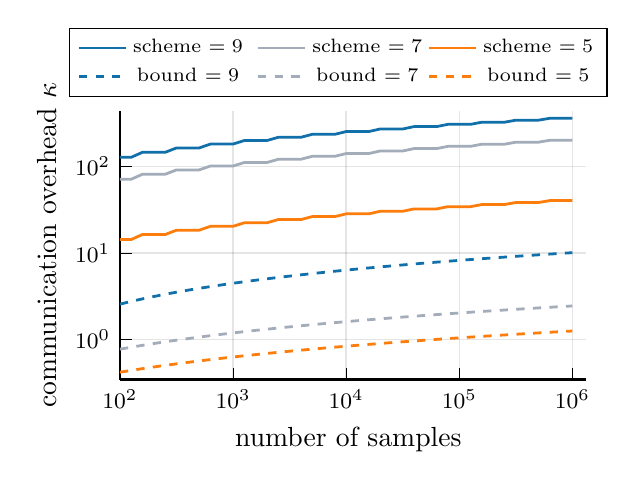
\begin{tikzpicture}
\begin{axis}[
  point meta max={nan}, 
  point meta min={nan}, 
  legend cell align={left}, 
  title={}, 
  title style={at={{(0.5,1)}}, anchor={south}, font={{\fontsize{14 pt}{18.2 pt}\selectfont}}, color={rgb,1:red,0.0;green,0.0;blue,0.0}, draw opacity={1.0}, rotate={0.0}}, 
  legend columns=3, 
  legend style={
            /tikz/column 2/.style={
                column sep=3pt,
            },
      font={{\fontsize{7 pt}{10.4 pt}\selectfont}},
      cells={anchor={center}},
      at={(-0.11,1.05)},
      anchor=south west
      }, 
  axis background/.style={fill={rgb,1:red,1.0;green,1.0;blue,1.0}, opacity={1.0}}, 
  anchor={north west}, 
  xshift={1.0mm}, 
  yshift={-1.0mm}, 
width={75mm}, 
height={50mm},
  xlabel={number of samples $\ngrad$}, 
  x tick style={color={rgb,1:red,0.0;green,0.0;blue,0.0}, opacity={1.0}}, 
  x tick label style={color={rgb,1:red,0.0;green,0.0;blue,0.0}, opacity={1.0}, rotate={0}}, 
  xmode={log}, 
  log basis x={10}, 
  xmajorgrids={true}, 
  xmin={100}, 
  xmax={1.3182567385564074e6}, 
  xtick={{100.0,1000.0,10000.0,100000.0,1.0e6}}, 
  xticklabels={{$10^{2}$,$10^{3}$,$10^{4}$,$10^{5}$,$10^{6}$}}, 
  xtick align={inside}, 
  xticklabel style={font={{\fontsize{8 pt}{10.4 pt}\selectfont}}, color={rgb,1:red,0.0;green,0.0;blue,0.0}, draw opacity={1.0}, rotate={0.0}}, 
  x grid style={color={rgb,1:red,0.0;green,0.0;blue,0.0}, draw opacity={0.1}, line width={0.5}, solid}, 
  axis x line*={left}, 
  x axis line style={color={rgb,1:red,0.0;green,0.0;blue,0.0}, draw opacity={1.0}, line width={1}, solid},  
  ylabel={communication overhead $\kappa$}, 
  y tick style={color={rgb,1:red,0.0;green,0.0;blue,0.0}, opacity={1.0}}, 
  y tick label style={color={rgb,1:red,0.0;green,0.0;blue,0.0}, opacity={1.0}, rotate={0}}, 
  ymode={log}, 
  log basis y={10}, 
  ymajorgrids={true}, 
  ymin={0.33891105976772384}, 
  ymax={443.60664700624926}, 
  ytick={{1.0,10.0,100.0}}, 
  yticklabels={{$10^{0}$,$10^{1}$,$10^{2}$}}, 
  ytick align={inside}, 
  yticklabel style={font={{\fontsize{8 pt}{10.4 pt}\selectfont}}, color={rgb,1:red,0.0;green,0.0;blue,0.0}, draw opacity={1.0}, rotate={0.0}}, 
  y grid style={color={rgb,1:red,0.0;green,0.0;blue,0.0}, draw opacity={0.1}, line width={0.5}, solid}, 
  axis y line*={left}, 
  y axis line style={color={rgb,1:red,0.0;green,0.0;blue,0.0}, draw opacity={1.0}, line width={1}, solid}, 
  colorbar={false}
  ]
  \addplot[color={rgb,1:red,0.0667;green,0.4392;blue,0.6667}, 
  name path={0e242e9c-d481-452f-a98b-d4d0f32d2b0d}, 
  draw opacity={1.0}, 
  line width={1},
  solid]
        table[row sep={\\}]
        {
            \\
            100.0  128.0625  \\
            126.0  128.0625  \\
            158.0  146.0625  \\
            200.0  146.0625  \\
            251.0  146.0625  \\
            316.0  164.0625  \\
            398.0  164.0625  \\
            501.0  164.0625  \\
            631.0  182.0625  \\
            794.0  182.0625  \\
            1000.0  182.0625  \\
            1259.0  200.0625  \\
            1585.0  200.0625  \\
            1995.0  200.0625  \\
            2512.0  218.0625  \\
            3162.0  218.0625  \\
            3981.0  218.0625  \\
            5012.0  236.0625  \\
            6310.0  236.0625  \\
            7943.0  236.0625  \\
            10000.0  254.0625  \\
            12589.0  254.0625  \\
            15849.0  254.0625  \\
            19953.0  272.0625  \\
            25119.0  272.0625  \\
            31623.0  272.0625  \\
            39811.0  290.0625  \\
            50119.0  290.0625  \\
            63096.0  290.0625  \\
            79433.0  308.0625  \\
            100000.0  308.0625  \\
            125893.0  308.0625  \\
            158489.0  326.0625  \\
            199526.0  326.0625  \\
            251189.0  326.0625  \\
            316228.0  344.0625  \\
            398107.0  344.0625  \\
            501187.0  344.0625  \\
            630957.0  362.0625  \\
            794328.0  362.0625  \\
            1.0e6  362.0625  \\
        }
        ;
    \addlegendentry {scheme $\nmalicious=9$}
    \addplot[color={rgb,1:red,0.6392;green,0.6745;blue,0.7255}, name path={5c6cc1ca-1ded-4112-8f2e-02f121141a9a}, draw opacity={1.0}, line width={1}, solid]
        table[row sep={\\}]
        {
            \\
            100.0  71.35416666666667  \\
            126.0  71.35416666666667  \\
            158.0  81.35416666666666  \\
            200.0  81.35416666666666  \\
            251.0  81.35416666666666  \\
            316.0  91.35416666666666  \\
            398.0  91.35416666666666  \\
            501.0  91.35416666666666  \\
            631.0  101.35416666666666  \\
            794.0  101.35416666666666  \\
            1000.0  101.35416666666666  \\
            1259.0  111.35416666666666  \\
            1585.0  111.35416666666666  \\
            1995.0  111.35416666666666  \\
            2512.0  121.35416666666666  \\
            3162.0  121.35416666666666  \\
            3981.0  121.35416666666666  \\
            5012.0  131.35416666666666  \\
            6310.0  131.35416666666666  \\
            7943.0  131.35416666666666  \\
            10000.0  141.35416666666666  \\
            12589.0  141.35416666666666  \\
            15849.0  141.35416666666666  \\
            19953.0  151.35416666666666  \\
            25119.0  151.35416666666666  \\
            31623.0  151.35416666666666  \\
            39811.0  161.35416666666669  \\
            50119.0  161.35416666666669  \\
            63096.0  161.35416666666669  \\
            79433.0  171.35416666666669  \\
            100000.0  171.35416666666669  \\
            125893.0  171.35416666666669  \\
            158489.0  181.35416666666669  \\
            199526.0  181.35416666666669  \\
            251189.0  181.35416666666669  \\
            316228.0  191.35416666666669  \\
            398107.0  191.35416666666669  \\
            501187.0  191.35416666666669  \\
            630957.0  201.35416666666669  \\
            794328.0  201.35416666666669  \\
            1.0e6  201.35416666666669  \\
        }
        ;
    \addlegendentry {scheme $\nmalicious=7$}
    \addplot[color={rgb,1:red,0.9882;green,0.4902;blue,0.0431}, name path={dfcf77df-a2d1-4ea1-845c-33668df8d22a}, draw opacity={1.0}, line width={1}, solid]
        table[row sep={\\}]
        {
            \\
            100.0  14.3125  \\
            126.0  14.3125  \\
            158.0  16.3125  \\
            200.0  16.3125  \\
            251.0  16.3125  \\
            316.0  18.3125  \\
            398.0  18.3125  \\
            501.0  18.3125  \\
            631.0  20.3125  \\
            794.0  20.3125  \\
            1000.0  20.3125  \\
            1259.0  22.3125  \\
            1585.0  22.3125  \\
            1995.0  22.3125  \\
            2512.0  24.3125  \\
            3162.0  24.3125  \\
            3981.0  24.3125  \\
            5012.0  26.3125  \\
            6310.0  26.3125  \\
            7943.0  26.3125  \\
            10000.0  28.3125  \\
            12589.0  28.3125  \\
            15849.0  28.3125  \\
            19953.0  30.3125  \\
            25119.0  30.3125  \\
            31623.0  30.3125  \\
            39811.0  32.3125  \\
            50119.0  32.3125  \\
            63096.0  32.3125  \\
            79433.0  34.3125  \\
            100000.0  34.3125  \\
            125893.0  34.3125  \\
            158489.0  36.3125  \\
            199526.0  36.3125  \\
            251189.0  36.3125  \\
            316228.0  38.3125  \\
            398107.0  38.3125  \\
            501187.0  38.3125  \\
            630957.0  40.3125  \\
            794328.0  40.3125  \\
            1.0e6  40.3125  \\
        }
        ;
    \addlegendentry {scheme $\nmalicious=5$}
    \addplot[color={rgb,1:red,0.0667;green,0.4392;blue,0.6667}, name path={916ac44c-4455-46cd-b337-0e0654368a75}, draw opacity={1.0}, line width={1}, dashed]
        table[row sep={\\}]
        {
            \\
            100.0  2.5494268877638664  \\
            126.0  2.7440371241983943  \\
            158.0  2.9331325267517325  \\
            200.0  3.128883048004122  \\
            251.0  3.3165914111458363  \\
            316.0  3.5061901440890875  \\
            398.0  3.6955659086180153  \\
            501.0  3.8840381331444855  \\
            631.0  4.072603223780094  \\
            794.0  4.260136076116884  \\
            1000.0  4.448177546208562  \\
            1259.0  4.635755271258833  \\
            1585.0  4.8231527834983625  \\
            1995.0  5.010272100836417  \\
            2512.0  5.197609674659617  \\
            3162.0  5.384626358943232  \\
            3981.0  5.571752991561537  \\
            5012.0  5.758814679803512  \\
            6310.0  5.945840686495122  \\
            7943.0  6.13272128263218  \\
            10000.0  6.319692701362235  \\
            12589.0  6.50660156695857  \\
            15849.0  6.693532947575442  \\
            19953.0  6.880445384325474  \\
            25119.0  7.067326362661656  \\
            31623.0  7.254212751333456  \\
            39811.0  7.441092356745352  \\
            50119.0  7.627966295589302  \\
            63096.0  7.814837009150257  \\
            79433.0  8.00170443437531  \\
            100000.0  8.18856949157318  \\
            125893.0  8.375437581178968  \\
            158489.0  8.562296747476802  \\
            199526.0  8.749160108488104  \\
            251189.0  8.936024004413222  \\
            316228.0  9.122884565235324  \\
            398107.0  9.309744183688146  \\
            501187.0  9.496604285418385  \\
            630957.0  9.683464008081398  \\
            794328.0  9.870323724796744  \\
            1.0e6  10.05718326043246  \\
        }
        ;
    \addlegendentry {bound $\nmalicious=9$}
    \addplot[color={rgb,1:red,0.6392;green,0.6745;blue,0.7255}, name path={18869fbd-03e6-4fe7-a510-983c69edb319}, draw opacity={1.0}, line width={1}, dashed]
        table[row sep={\\}]
        {
            \\
            100.0  0.7670758006158959  \\
            126.0  0.8089415130101252  \\
            158.0  0.8499000935667956  \\
            200.0  0.8925300506448983  \\
            251.0  0.9335829899133037  \\
            316.0  0.9751867979102739  \\
            398.0  1.016851238605413  \\
            501.0  1.058403192366081  \\
            631.0  1.1000440133356142  \\
            794.0  1.1415107658029335  \\
            1000.0  1.1831328220284065  \\
            1259.0  1.2246861734123942  \\
            1585.0  1.2662264840691486  \\
            1995.0  1.307726420344244  \\
            2512.0  1.3492916913851953  \\
            3162.0  1.3907991857664292  \\
            3981.0  1.4323417419701476  \\
            5012.0  1.4738783451094648  \\
            6310.0  1.515413745332678  \\
            7943.0  1.5569221833427682  \\
            10000.0  1.5984550301488034  \\
            12589.0  1.6399773456751503  \\
            15849.0  1.681507335010188  \\
            19953.0  1.7230352378837055  \\
            25119.0  1.7645578365912284  \\
            31623.0  1.8060829759536532  \\
            39811.0  1.8476076713134992  \\
            50119.0  1.889131952033178  \\
            63096.0  1.9306561868386218  \\
            79433.0  1.9721802237317847  \\
            100000.0  2.0137041576156927  \\
            125893.0  2.055229101501116  \\
            158489.0  2.0967523294952826  \\
            199526.0  2.138276701715617  \\
            251189.0  2.179801361275636  \\
            316228.0  2.2213254135319436  \\
            398107.0  2.2628493626695687  \\
            501187.0  2.3043735036336517  \\
            630957.0  2.345897627428272  \\
            794328.0  2.387421803174363  \\
            1.0e6  2.4289459809970366  \\
        }
        ;
    \addlegendentry {bound $\nmalicious=7$}
    \addplot[color={rgb,1:red,0.9882;green,0.4902;blue,0.0431}, name path={a9e21dfe-363f-47d4-9a89-d46c55fb56ce}, draw opacity={1.0}, line width={1}, dashed]
        table[row sep={\\}]
        {
            \\
            100.0  0.4152410118609203  \\
            126.0  0.4360799952187448  \\
            158.0  0.45648629676106894  \\
            200.0  0.4777410118609203  \\
            251.0  0.49822147212192325  \\
            316.0  0.5189862967610689  \\
            398.0  0.5397890387839781  \\
            501.0  0.5605416745747005  \\
            631.0  0.5813435121864093  \\
            794.0  0.6020621998214348  \\
            1000.0  0.6228615177913804  \\
            1259.0  0.6436289104824385  \\
            1585.0  0.6643916953141731  \\
            1995.0  0.6851358144443568  \\
            2512.0  0.7059137968057266  \\
            3162.0  0.7266638532723981  \\
            3981.0  0.7474321972557093  \\
            5012.0  0.7681981687076163  \\
            6310.0  0.7889640181168694  \\
            7943.0  0.8097167679974888  \\
            10000.0  0.8304820237218405  \\
            12589.0  0.8512422542189988  \\
            15849.0  0.872006512204595  \\
            19953.0  0.8927698785193512  \\
            25119.0  0.9135307131567737  \\
            31623.0  0.9342929136775154  \\
            39811.0  0.9550549681273297  \\
            50119.0  0.9758168755690503  \\
            63096.0  0.9965788079587001  \\
            79433.0  1.0173406794449065  \\
            100000.0  1.0381025296523008  \\
            125893.0  1.0588649088673643  \\
            158489.0  1.079626449211309  \\
            199526.0  1.100388576814992  \\
            251189.0  1.1211508601214328  \\
            316228.0  1.1419128493349135  \\
            398107.0  1.1626747945814155  \\
            501187.0  1.1834368417718029  \\
            630957.0  1.2041988851679049  \\
            794328.0  1.2249609583449041  \\
            1.0e6  1.2457230355827609  \\
        }
        ;
    \addlegendentry {bound $\nmalicious=5$}
\end{axis}
\end{tikzpicture}

    }
    \caption{Comparison of converse and achievability for $\commoh$ over the dataset size $\ngrad$. We consider a system of $\nworker=10$ workers, $\ngroup=1$ group and an alphabet size $|\galpha|=2^{16}$. As the percentage of malicious workers rises from \SI{50}{\percent} to \SI{90}{\percent} the communication overhead of the scheme increases. }
    \label{fig:achievability_vs_converse_datacolumns}
\end{figure}

The gap between our scheme and the bound is depicted in~\cref{fig:achievability_vs_converse_datacolumns}.
It shows that for any parameter $\nmalicious$, the scheme is a constant factor away from the bound.
Typically, in distributed gradient descent applications the number of parameters $\graddim$ and the number of samples $\ngrad$ are very large, whereas the number of workers $\nworker$ and as a consequence $\nmalicious$, $\nhonest$ and $\ngroup$ are small by comparison.
For large numbers of samples $\ngrad$, the ratio $\commoh[achieve]/\commoh[bound]$ tends to 
\begin{align}
  \label{eq:conv_limit}
\lim_{\ngrad \to \infty} \frac{\commoh[achieve]}{\commoh[bound]} &= 2 \log_2(|\galpha|) \frac{(\nmalicious - \nhonest + 1)}{\lfloor \nmalicious / \nhonest 
\rfloor}.
\end{align}

The convergence behavior can be observed in \cref{fig:convergence}.
\begin{figure}[h]
    \centering
    \resizebox{0.98\linewidth}{!}{
    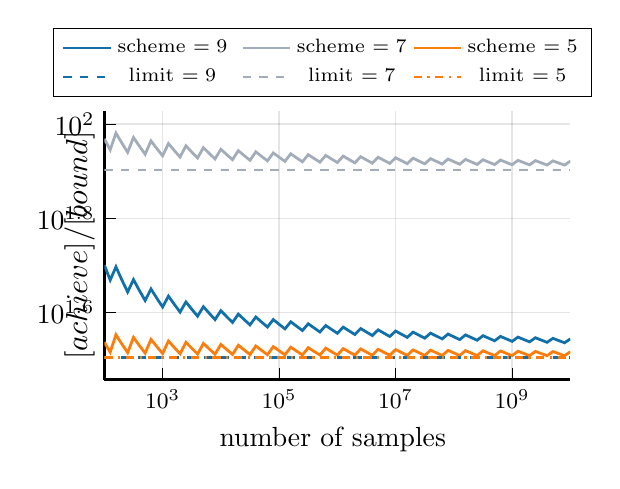
\begin{tikzpicture}
\begin{axis}[
  legend cell align={left}, 
  legend columns={3}, 
  title style={at={{(0.1,1)}}, anchor={south}, font={{\fontsize{14 pt}{18.2 pt}\selectfont}}, color={rgb,1:red,0.0;green,0.0;blue,0.0}, draw opacity={1.0}, rotate={0.0}}, 
    legend style={
            /tikz/column 2/.style={
                column sep=3pt,
            },
      font={{\fontsize{7 pt}{10.4 pt}\selectfont}},
      cells={anchor={center}},
      at={(-0.11,1.05)},
      anchor=south west
      }, 
  axis background/.style={fill={rgb,1:red,1.0;green,1.0;blue,1.0}, opacity={1.0}}, 
  anchor={north west}, 
  xshift={1.0mm}, 
  yshift={-1.0mm}, 
  width={75mm}, 
  height={50mm}, 
  xlabel={number of samples $\ngrad$}, 
  x tick style={color={rgb,1:red,0.0;green,0.0;blue,0.0}, opacity={1.0}}, 
  x tick label style={color={rgb,1:red,0.0;green,0.0;blue,0.0}, opacity={1.0}, rotate={0}}, 
  xmode={log}, 
  log basis x={10}, 
  xmajorgrids={true}, 
  xmin={100}, 
  xmax={1e10}, 
  xticklabel style={font={{\fontsize{8 pt}{10.4 pt}\selectfont}}, color={rgb,1:red,0.0;green,0.0;blue,0.0}, draw opacity={1.0}, rotate={0.0}}, 
  x grid style={color={rgb,1:red,0.0;green,0.0;blue,0.0}, draw opacity={0.1}, line width={0.5}, solid}, 
  axis x line*={left}, 
  x axis line style={color={rgb,1:red,0.0;green,0.0;blue,0.0}, draw opacity={1.0}, line width={1}, solid}, 
  scaled y ticks={false}, 
  ylabel={$\commoh[achieve] / \commoh[bound]$}, 
  y tick style={color={rgb,1:red,0.0;green,0.0;blue,0.0}, opacity={1.0}}, 
  y tick label style={color={rgb,1:red,0.0;green,0.0;blue,0.0}, opacity={1.0}, rotate={0}}, 
  ylabel style={at={(0, 0.5)},
   font={{\fontsize{11 pt}{14.3 pt}\selectfont}}, color={rgb,1:red,0.0;green,0.0;blue,0.0}, draw opacity={1.0}, rotate={0.0}}, 
  ymode={log}, 
  log basis y={10}, 
  ymajorgrids={true}, 
  ytick align={inside}, 
  y grid style={color={rgb,1:red,0.0;green,0.0;blue,0.0}, draw opacity={0.1}, line width={0.5}, solid}, 
  axis y line*={left}, 
  y axis line style={color={rgb,1:red,0.0;green,0.0;blue,0.0}, draw opacity={1.0}, line width={1}, solid}, 
  colorbar={false}]
    
  \addplot[color={rgb,1:red,0.0667;green,0.4392;blue,0.6667}, 
  name path={1eeefe02-17e6-4c94-a00a-326681316fae}, 
  draw opacity={1.0}, 
  line width={1}, solid]
        table[row sep={\\}]
        {
            \\
            100.0  50.23187784464185  \\
            126.0  46.66937588805779  \\
            158.0  49.797443063970725  \\
            200.0  46.68199410430874  \\
            251.0  44.03994399465005  \\
            316.0  46.792242650212465  \\
            398.0  44.39441862406194  \\
            501.0  42.24018775716199  \\
            631.0  44.704207602874185  \\
            794.0  42.73631094102282  \\
            1000.0  40.92968369825578  \\
            1259.0  43.15639810418062  \\
            1585.0  41.47961074019498  \\
            1995.0  39.93046604526758  \\
            2512.0  41.954381658003314  \\
            3162.0  40.49723889157579  \\
            3981.0  39.13714415019067  \\
            5012.0  40.99150834422307  \\
            6310.0  39.70212329034855  \\
            7943.0  38.49229226648979  \\
            10000.0  40.20171739446062  \\
            12589.0  39.04688144578651  \\
            15849.0  37.95641285250228  \\
            19953.0  39.541408266940515  \\
            25119.0  38.495816669422545  \\
            31623.0  37.504069611135954  \\
            39811.0  38.981171862093376  \\
            50119.0  38.026190567690634  \\
            63096.0  37.116896956439504  \\
            79433.0  38.49960999266156  \\
            100000.0  37.62103995295219  \\
            125893.0  36.781660303011364  \\
            158489.0  38.08119592398925  \\
            199526.0  37.26786296705972  \\
            251189.0  36.48854343262372  \\
            316228.0  37.71422268249702  \\
            398107.0  36.957245356197994  \\
            501187.0  36.23005546606724  \\
            630957.0  37.38977081939256  \\
            794328.0  36.681927573500715  \\
            1.0e6  36.00038804348399  \\
            1.258925e6  37.10083340384379  \\
            1.584893e6  36.43620911979894  \\
            1.995262e6  35.79497895914034  \\
            2.511886e6  36.841882515756005  \\
            3.162278e6  36.21555769415743  \\
            3.981072e6  35.61017335620257  \\
            5.011872e6  36.60847880764624  \\
            6.309573e6  36.01632360927727  \\
            7.943282e6  35.443020129509705  \\
            1.0e7  36.397018661122004  \\
            1.2589254e7  35.83553091978193  \\
            1.5848932e7  35.291103835461016  \\
            1.9952623e7  36.20454620521198  \\
            2.5118864e7  35.67073279485513  \\
            3.1622777e7  35.15243210067665  \\
            3.9810717e7  36.028613528596004  \\
            5.0118723e7  35.51989633552601  \\
            6.3095734e7  35.0253450987719  \\
            7.9432823e7  35.867176452423976  \\
            1.0e8  35.38131934771668  \\
            1.25892541e8  34.90844919089674  \\
            1.58489319e8  35.71851428074481  \\
            1.99526231e8  35.25356557796952  \\
            2.51188643e8  34.80056582737158  \\
            3.16227766e8  35.58116836540663  \\
            3.98107171e8  35.13541465660039  \\
            5.01187234e8  34.70069138989681  \\
            6.30957344e8  35.453893970266584  \\
            7.94328235e8  35.025823089174395  \\
            1.0e9  34.6079659594997  \\
            1.258925412e9  35.33562245455053  \\
            1.584893192e9  34.92389326404258  \\
            1.995262315e9  34.5216484632405  \\
            2.511886432e9  35.22543120976006  \\
            3.16227766e9  34.82884884642847  \\
            3.981071706e9  34.4410968407726  \\
            5.011872336e9  35.122519523880754  \\
            6.309573445e9  34.74001496234031  \\
            7.943282347e9  34.365752036937266  \\
            1.0e10  35.0261890975617  \\
        }
        ;
    \addlegendentry {scheme $\nmalicious=9$}
    \addplot[color={rgb,1:red,0.6392;green,0.6745;blue,0.7255},  draw opacity={1.0}, line width={1}, solid]
        table[row sep={\\}]
        {
            \\
            100.0  93.02101123432054  \\
            126.0  88.206830183746  \\
            158.0  95.7220351926845  \\
            200.0  91.15005887799984  \\
            251.0  87.14186906321154  \\
            316.0  93.6786335319852  \\
            398.0  89.84024722432035  \\
            501.0  86.31320022990731  \\
            631.0  92.13646493955724  \\
            794.0  88.78949695702133  \\
            1000.0  85.66592421373394  \\
            1259.0  90.92465407394606  \\
            1585.0  87.94174507298143  \\
            1995.0  85.1509650140386  \\
            2512.0  89.93916396393381  \\
            3162.0  87.25498828919135  \\
            3981.0  84.72431062418615  \\
            5012.0  89.12144418331283  \\
            6310.0  86.67874834263863  \\
            7943.0  84.36784321785724  \\
            10000.0  88.43174440353678  \\
            12589.0  86.19275567399598  \\
            15849.0  84.06396078302579  \\
            19953.0  87.84159681642109  \\
            25119.0  85.77455696156296  \\
            31623.0  83.80244356533409  \\
            39811.0  87.33140112584451  \\
            50119.0  85.41180328510632  \\
            63096.0  83.57478030869814  \\
            79433.0  86.88565304768554  \\
            100000.0  85.09401245392321  \\
            125893.0  83.3747276843791  \\
            158489.0  86.49288908162137  \\
            199526.0  84.81323606115133  \\
            251189.0  83.1975655619083  \\
            316228.0  86.14413966588103  \\
            398107.0  84.56336945068185  \\
            501187.0  83.03956210437667  \\
            630957.0  85.8324610215001  \\
            794328.0  84.33958607521396  \\
            1.0e6  82.8977541048544  \\
            1.258925e6  85.5522079182146  \\
            1.584893e6  84.13799964535005  \\
            1.995262e6  82.76978730817473  \\
            2.511886e6  85.29886289954584  \\
            3.162278e6  83.9554628949764  \\
            3.981072e6  82.65372387547478  \\
            5.011872e6  85.06872773786297  \\
            6.309573e6  83.78939956634181  \\
            7.943282e6  82.5479801722578  \\
            1.0e7  84.85875239086057  \\
            1.2589254e7  83.63767265672266  \\
            1.5848932e7  82.45123590472062  \\
            1.9952623e7  84.66639913616976  \\
            2.5118864e7  83.49850377095927  \\
            3.1622777e7  82.36238995668099  \\
            3.9810717e7  84.48953848435559  \\
            5.0118723e7  83.37039542564209  \\
            6.3095734e7  82.28051295295855  \\
            7.9432823e7  84.32637126029363  \\
            1.0e8  83.25207945755008  \\
            1.25892541e8  82.2048156496943  \\
            1.58489319e8  84.17536632011632  \\
            1.99526231e8  83.14247447216985  \\
            2.51188643e8  82.13462397810892  \\
            3.16227766e8  84.03521272321055  \\
            3.98107171e8  83.04065254291943  \\
            5.01187234e8  82.06935833654543  \\
            6.30957344e8  83.90478135456816  \\
            7.94328235e8  82.94581312045894  \\
            1.0e9  82.00851775215477  \\
            1.258925412e9  83.78309448643056  \\
            1.584893192e9  82.85726175304116  \\
            1.995262315e9  81.95166693685219  \\
            2.511886432e9  83.66930126432923  \\
            3.16227766e9  82.7743931365518  \\
            3.981071706e9  81.89842589399396  \\
            5.011872336e9  83.5626577416165  \\
            6.309573445e9  82.69667724875488  \\
            7.943282347e9  81.84846139720672  \\
            1.0e10  83.46251060976827  \\
        }
        ;
    \addlegendentry {scheme $\nmalicious=7$}
    \addplot[color={rgb,1:red,0.9882;green,0.4902;blue,0.0431}, name path={44590de5-03d4-4a3a-937b-5ede02b3c2bf}, draw opacity={1.0}, line width={1}, solid]
        table[row sep={\\}]
        {
            \\
            100.0  34.467934503525846  \\
            126.0  32.820813054771335  \\
            158.0  35.73491716124434  \\
            200.0  34.14506938907913  \\
            251.0  32.74146321017665  \\
            316.0  35.28513202426752  \\
            398.0  33.92529059362506  \\
            501.0  32.669292633583815  \\
            631.0  34.94061527169283  \\
            794.0  33.73820845425019  \\
            1000.0  32.61158286359796  \\
            1259.0  34.666714991524294  \\
            1585.0  33.583351744709894  \\
            1995.0  32.56653575772473  \\
            2512.0  34.44117413487953  \\
            3162.0  33.45769834361939  \\
            3981.0  32.528034100305526  \\
            5012.0  34.25222953117296  \\
            6310.0  33.350697111388826  \\
            7943.0  32.49593072534914  \\
            10000.0  34.09164700894587  \\
            12589.0  33.260214539016594  \\
            15849.0  32.46822082603572  \\
            19953.0  33.95331846351373  \\
            25119.0  33.181697739808754  \\
            31623.0  32.444321856927615  \\
            39811.0  33.83313115826024  \\
            50119.0  33.11328263426156  \\
            63096.0  32.42342676961588  \\
            79433.0  33.72763980962798  \\
            100000.0  33.05309352390513  \\
            125893.0  32.40498359389683  \\
            158489.0  33.63431863541976  \\
            199526.0  32.99970643561598  \\
            251189.0  32.388593981069555  \\
            316228.0  33.55115937465317  \\
            398107.0  32.95203454874345  \\
            501187.0  32.37392875367965  \\
            630957.0  33.47661295532516  \\
            794328.0  32.909212106211044  \\
            1.0e6  32.36072453387798  \\
            1.258925e6  33.40939537878277  \\
            1.584893e6  32.87053367710583  \\
            1.995262e6  32.34877925115103  \\
            2.511886e6  33.34847959590082  \\
            3.162278e6  32.83542544512263  \\
            3.981072e6  32.33791907378289  \\
            5.011872e6  33.2930190682296  \\
            6.309573e6  32.80341585166549  \\
            7.943282e6  32.32800397112567  \\
            1.0e7  33.242312378322495  \\
            1.2589254e7  32.774110814310454  \\
            1.5848932e7  32.31891480298508  \\
            1.9952623e7  33.19577350926881  \\
            2.5118864e7  32.74718198485234  \\
            3.1622777e7  32.310552844367464  \\
            3.9810717e7  33.15290873562767  \\
            5.0118723e7  32.72235149007836  \\
            6.3095734e7  32.302834162867505  \\
            7.9432823e7  33.11329953386461  \\
            1.0e8  32.69938327899996  \\
            1.25892541e8  32.29568719160354  \\
            1.58489319e8  33.07658855067729  \\
            1.99526231e8  32.67807543717949  \\
            2.51188643e8  32.289050726389824  \\
            3.16227766e8  33.04246893591277  \\
            3.98107171e8  32.65825417890546  \\
            5.01187234e8  32.28287194759399  \\
            6.30957344e8  33.01067566211962  \\
            7.94328235e8  32.639769192227135  \\
            1.0e9  32.27710509063798  \\
            1.258925412e9  32.98097864556565  \\
            1.584893192e9  32.62248974794688  \\
            1.995262315e9  32.2717102878248  \\
            2.511886432e9  32.953177184621545  \\
            3.16227766e9  32.606301635683224  \\
            3.981071706e9  32.266652660062476  \\
            5.011872336e9  32.92709540208889  \\
            6.309573445e9  32.59110463255507  \\
            7.943282347e9  32.2619015555467  \\
            1.0e10  32.90257852607314  \\
        }
        ;
    \addlegendentry {scheme $\nmalicious=5$}
    \addplot[color={rgb,1:red,0.0667;green,0.4392;blue,0.6667}, name path={233b7f50-a717-44f1-9f9e-0bb573127f34}, draw opacity={1.0}, line width={1}, thick, dashed]
        table[row sep={\\}]
        {
            \\
            100.0  32.0  \\
            126.0  32.0  \\
            158.0  32.0  \\
            200.0  32.0  \\
            251.0  32.0  \\
            316.0  32.0  \\
            398.0  32.0  \\
            501.0  32.0  \\
            631.0  32.0  \\
            794.0  32.0  \\
            1000.0  32.0  \\
            1259.0  32.0  \\
            1585.0  32.0  \\
            1995.0  32.0  \\
            2512.0  32.0  \\
            3162.0  32.0  \\
            3981.0  32.0  \\
            5012.0  32.0  \\
            6310.0  32.0  \\
            7943.0  32.0  \\
            10000.0  32.0  \\
            12589.0  32.0  \\
            15849.0  32.0  \\
            19953.0  32.0  \\
            25119.0  32.0  \\
            31623.0  32.0  \\
            39811.0  32.0  \\
            50119.0  32.0  \\
            63096.0  32.0  \\
            79433.0  32.0  \\
            100000.0  32.0  \\
            125893.0  32.0  \\
            158489.0  32.0  \\
            199526.0  32.0  \\
            251189.0  32.0  \\
            316228.0  32.0  \\
            398107.0  32.0  \\
            501187.0  32.0  \\
            630957.0  32.0  \\
            794328.0  32.0  \\
            1.0e6  32.0  \\
            1.258925e6  32.0  \\
            1.584893e6  32.0  \\
            1.995262e6  32.0  \\
            2.511886e6  32.0  \\
            3.162278e6  32.0  \\
            3.981072e6  32.0  \\
            5.011872e6  32.0  \\
            6.309573e6  32.0  \\
            7.943282e6  32.0  \\
            1.0e7  32.0  \\
            1.2589254e7  32.0  \\
            1.5848932e7  32.0  \\
            1.9952623e7  32.0  \\
            2.5118864e7  32.0  \\
            3.1622777e7  32.0  \\
            3.9810717e7  32.0  \\
            5.0118723e7  32.0  \\
            6.3095734e7  32.0  \\
            7.9432823e7  32.0  \\
            1.0e8  32.0  \\
            1.25892541e8  32.0  \\
            1.58489319e8  32.0  \\
            1.99526231e8  32.0  \\
            2.51188643e8  32.0  \\
            3.16227766e8  32.0  \\
            3.98107171e8  32.0  \\
            5.01187234e8  32.0  \\
            6.30957344e8  32.0  \\
            7.94328235e8  32.0  \\
            1.0e9  32.0  \\
            1.258925412e9  32.0  \\
            1.584893192e9  32.0  \\
            1.995262315e9  32.0  \\
            2.511886432e9  32.0  \\
            3.16227766e9  32.0  \\
            3.981071706e9  32.0  \\
            5.011872336e9  32.0  \\
            6.309573445e9  32.0  \\
            7.943282347e9  32.0  \\
            1.0e10  32.0  \\
        }
        ;
      \addlegendentry {limit $\nmalicious=9$}
    \addplot[color={rgb,1:red,0.6392;green,0.6745;blue,0.7255}, name path={f75f2af8-a259-464f-ac67-414608860373}, draw opacity={1.0}, line width={1}, thick, dashed]
        table[row sep={\\}]
        {
            \\
            100.0  80.0  \\
            126.0  80.0  \\
            158.0  80.0  \\
            200.0  80.0  \\
            251.0  80.0  \\
            316.0  80.0  \\
            398.0  80.0  \\
            501.0  80.0  \\
            631.0  80.0  \\
            794.0  80.0  \\
            1000.0  80.0  \\
            1259.0  80.0  \\
            1585.0  80.0  \\
            1995.0  80.0  \\
            2512.0  80.0  \\
            3162.0  80.0  \\
            3981.0  80.0  \\
            5012.0  80.0  \\
            6310.0  80.0  \\
            7943.0  80.0  \\
            10000.0  80.0  \\
            12589.0  80.0  \\
            15849.0  80.0  \\
            19953.0  80.0  \\
            25119.0  80.0  \\
            31623.0  80.0  \\
            39811.0  80.0  \\
            50119.0  80.0  \\
            63096.0  80.0  \\
            79433.0  80.0  \\
            100000.0  80.0  \\
            125893.0  80.0  \\
            158489.0  80.0  \\
            199526.0  80.0  \\
            251189.0  80.0  \\
            316228.0  80.0  \\
            398107.0  80.0  \\
            501187.0  80.0  \\
            630957.0  80.0  \\
            794328.0  80.0  \\
            1.0e6  80.0  \\
            1.258925e6  80.0  \\
            1.584893e6  80.0  \\
            1.995262e6  80.0  \\
            2.511886e6  80.0  \\
            3.162278e6  80.0  \\
            3.981072e6  80.0  \\
            5.011872e6  80.0  \\
            6.309573e6  80.0  \\
            7.943282e6  80.0  \\
            1.0e7  80.0  \\
            1.2589254e7  80.0  \\
            1.5848932e7  80.0  \\
            1.9952623e7  80.0  \\
            2.5118864e7  80.0  \\
            3.1622777e7  80.0  \\
            3.9810717e7  80.0  \\
            5.0118723e7  80.0  \\
            6.3095734e7  80.0  \\
            7.9432823e7  80.0  \\
            1.0e8  80.0  \\
            1.25892541e8  80.0  \\
            1.58489319e8  80.0  \\
            1.99526231e8  80.0  \\
            2.51188643e8  80.0  \\
            3.16227766e8  80.0  \\
            3.98107171e8  80.0  \\
            5.01187234e8  80.0  \\
            6.30957344e8  80.0  \\
            7.94328235e8  80.0  \\
            1.0e9  80.0  \\
            1.258925412e9  80.0  \\
            1.584893192e9  80.0  \\
            1.995262315e9  80.0  \\
            2.511886432e9  80.0  \\
            3.16227766e9  80.0  \\
            3.981071706e9  80.0  \\
            5.011872336e9  80.0  \\
            6.309573445e9  80.0  \\
            7.943282347e9  80.0  \\
            1.0e10  80.0  \\
        }
        ;
        \addlegendentry {limit $\nmalicious=7$}
    \addplot[color={rgb,1:red,0.9882;green,0.4902;blue,0.0431}, name path={6095e951-ac26-4dd8-b5f0-843e048439e3}, draw opacity={1.0}, line width={1}, thick, dashdotted]
        table[row sep={\\}]
        {
            \\
            100.0  32.0  \\
            126.0  32.0  \\
            158.0  32.0  \\
            200.0  32.0  \\
            251.0  32.0  \\
            316.0  32.0  \\
            398.0  32.0  \\
            501.0  32.0  \\
            631.0  32.0  \\
            794.0  32.0  \\
            1000.0  32.0  \\
            1259.0  32.0  \\
            1585.0  32.0  \\
            1995.0  32.0  \\
            2512.0  32.0  \\
            3162.0  32.0  \\
            3981.0  32.0  \\
            5012.0  32.0  \\
            6310.0  32.0  \\
            7943.0  32.0  \\
            10000.0  32.0  \\
            12589.0  32.0  \\
            15849.0  32.0  \\
            19953.0  32.0  \\
            25119.0  32.0  \\
            31623.0  32.0  \\
            39811.0  32.0  \\
            50119.0  32.0  \\
            63096.0  32.0  \\
            79433.0  32.0  \\
            100000.0  32.0  \\
            125893.0  32.0  \\
            158489.0  32.0  \\
            199526.0  32.0  \\
            251189.0  32.0  \\
            316228.0  32.0  \\
            398107.0  32.0  \\
            501187.0  32.0  \\
            630957.0  32.0  \\
            794328.0  32.0  \\
            1.0e6  32.0  \\
            1.258925e6  32.0  \\
            1.584893e6  32.0  \\
            1.995262e6  32.0  \\
            2.511886e6  32.0  \\
            3.162278e6  32.0  \\
            3.981072e6  32.0  \\
            5.011872e6  32.0  \\
            6.309573e6  32.0  \\
            7.943282e6  32.0  \\
            1.0e7  32.0  \\
            1.2589254e7  32.0  \\
            1.5848932e7  32.0  \\
            1.9952623e7  32.0  \\
            2.5118864e7  32.0  \\
            3.1622777e7  32.0  \\
            3.9810717e7  32.0  \\
            5.0118723e7  32.0  \\
            6.3095734e7  32.0  \\
            7.9432823e7  32.0  \\
            1.0e8  32.0  \\
            1.25892541e8  32.0  \\
            1.58489319e8  32.0  \\
            1.99526231e8  32.0  \\
            2.51188643e8  32.0  \\
            3.16227766e8  32.0  \\
            3.98107171e8  32.0  \\
            5.01187234e8  32.0  \\
            6.30957344e8  32.0  \\
            7.94328235e8  32.0  \\
            1.0e9  32.0  \\
            1.258925412e9  32.0  \\
            1.584893192e9  32.0  \\
            1.995262315e9  32.0  \\
            2.511886432e9  32.0  \\
            3.16227766e9  32.0  \\
            3.981071706e9  32.0  \\
            5.011872336e9  32.0  \\
            6.309573445e9  32.0  \\
            7.943282347e9  32.0  \\
            1.0e10  32.0  \\
        }
        ;
        \addlegendentry {limit $\nmalicious=5$}
\end{axis}
\end{tikzpicture}

    }
    \caption{Convergence of the ratio $\frac{\commoh[achieve]}{\commoh[bound]}$ to the limit given in $\eqref{eq:conv_limit}$ for large numbers of samples.
      The parameters are $\nworker=10$, $\ngroup=10$, $|\galpha|=2^{16}$.
    For $\nmalicious=5$ and $\nmalicious=9$ the limits as in \eqref{eq:conv_limit} yield the same value.}
    \label{fig:convergence}
\end{figure}
Note that depending on the alphabet the communication overhead of our scheme can be slightly improved as stated in the following.
\begin{remark}[Compression Beyond the Alphabet Size]
  If for every pair of elements $a, b \in \galpha$ there exists a
  function $f: \galpha \mapsto \mathcal{B}$, that maps from $\galpha$ to a
smaller alphabet $\mathcal{B}$, such that $f(a) \neq f(b)$ and an operation $\oplus$ with the property $\forall c, d, e, g \in \galpha: f(c+d) \neq f(e+g) \implies f(c) \neq f(d)\text{ or }f(e) \neq f(g)$, then 
our scheme can be improved to $\commoh \geq \left(\nmalicious+1-\nhonest\right) \left( 2 \lceil \log_{|\galpha|}(|\mathcal{B}|)\rceil \left\lceil \log_2\left( \frac{\ngrad}{\ngroup}\right) \right\rceil+ \frac{\nmalicious+3\nhonest}{2\log_2{\card{\galpha}}} \right)$.
At the start of each match, the main node chooses not only the index $\compind$ but also the appropriate function $f$ and communicates it to the two workers. They then use $f$ to compress their transmitted symbols during the match. 
\end{remark}





\pagebreak
\subsection{Notation}
\label{app:notations}
% \documentclass[a4paper]{amsart}%[a4paper]
% %%%%% GENERAL MATH COMMANDS
% Reals
\newcommand{\R}{{\mathbb R}}
% Integers
\newcommand{\Z}{{\mathbb Z}}
% Naturals
\newcommand{\N}{{\mathbb N}}
% Expectation
\DeclareMathOperator*{\E}{\mathbb{E}}
% ^th notation
\newcommand{\tth}{^{\text{th}}}
% Small dots for integer range [a .. b]
\newcommand{\sdots}{\,..\,}
% Vectorized version of matrix
\newcommand{\matvec}{\mbox{vec}}

% := sign
\newcommand{\defeq}{\vcentcolon=}
% Zero function
\newcommand{\zf}{\mathbf{0}}
% Vector of ones
\newcommand{\ones}{\mathbf{1}}

% Argmin and argmax definitions
\DeclareMathOperator*{\argmax}{arg\,max}
\DeclareMathOperator*{\argmin}{arg\,min}


%%%%% PROBLEM STATEMENT NOTATION 
% \newcommandtwoopt{\St}[2][t][]{{S_{#1}^{#2}}} % State
\newcommand{\task}[1][i]{{\mathcal{T}_{#1}}} % Task, optionally takes index
\newcommand{\tasks}{\{ \task \}_{i=1}^N}
\newcommand{\losst}[1][i]{{l_{#1}}}
\newcommand{\lossv}[1][i]{{l_{#1}^{\textrm{val}}}}
\newcommand{\tasktarget}{{\mathcal{T}_{\textrm{target}}}}
\newcommand{\lossttarget}{l_{\textrm{target}}}
\newcommand{\lossvtarget}{l_{\textrm{target}}^{\textrm{val}}}
\newcommand{\lossttargetit}{l_{\textrm{target}}^{(k)}}
\newcommand{\losstotal}{l^{\textrm{total}}}
\newcommand{\lossopt}{l^*}

\newcommand{\thetait}[2]{\theta_{#1}^{(#2)}}
\newcommand{\phit}[1]{\phi^{(#1)}}
\newcommand{\hist}[2]{S_{#1}^{(#2)}}
\newcommand{\grad}[2]{G_{#1}^{(#2)}}

\newcommand{\Alg}{\textup{\textbf{Opt}}}
\newcommand{\MetaAlg}{\textup{\textbf{MetaOpt}}}

%%%%% Theorems
\newtheoremstyle{mytheoremstyle} % name
    {\topsep}                    % Space above
    {\topsep}                    % Space below
    {\itshape}                   % Body font
    {}                           % Indent amount
    {\scshape}                   % Theorem head font
    {.}                          % Punctuation after theorem head
    {.5em}                       % Space after theorem head
    {}  % Theorem head spec (can be left empty, meaning ‘normal’)
\theoremstyle{mytheoremstyle}
\theoremstyle{plain}
\newtheorem{theorem}{Theorem}
\newtheorem{proposition}{Proposition}
\newtheorem{assumption}{Assumption}
\newtheorem{definition}{Definition}
\newtheorem{lemma}{Lemma}
\theoremstyle{remark}
\newtheorem{remark}{Remark}

%
% \begin{document}
% \section{notation}\label{sec:notation}
For a positive integer $d$, we define $[d]:=\{1,2,\ldots,d\}$. 
The set of non-negative integers is denoted by $\NN:=\{0,1,2,\ldots\}$.
The cardinality of a set $S$ is denoted by $|S|$.
%Operations on $[d]$ cyclically.

Our \emph{graphs} are finite and undirected. We allow multiple edges and loops. A \emph{simple graph} is a graph without multiple edges or loops. 


A \emph{plane map} is a connected planar graph drawn in the plane without edge crossing, considered up to continuous deformation. 
The \emph{faces} of a plane map are the connected components of the complement of the graph. The infinite face is called \emph{outer face}, and the finite faces are called \emph{inner faces}. The vertices and edges incident to the outer face are called \emph{outer} while the other are called \emph{inner}. 
The numbers $\vv$, $\ee$ and $\ff$ of vertices, edges and faces of a plane map are related by the \emph{Euler relation}  $\vv+\ff=\ee+2$. 


We now define the class of plane maps which will be relevant for this article.
\begin{definition}\label{def:d-adapted}
A \emph{$d$-map} is a plane map such that the inner faces have degree at most $d$, and the outer face has degree $d$ and is incident to $d$ distinct vertices (in other words, the contour of the outer face is a simple cycle). 
We will assume that the outer vertices of a $d$-map are labeled $v_1,v_2,\ldots, v_d$ in clockwise order along the boundary of the outer face. %, as in Figure \ref{???}.\\
A \emph{$d$-adapted map} is a $d$-map such that any simple cycle which is not the contour of a face has length at least $d$.\\
\end{definition}
We point out that $d$-adapted maps are necessarily 2-connected (because a cut point in a $d$-map $G$ implies the existence of a simple cycle of length strictly less than the degree of an inner face of $G$, which shows that $G$ is not $d$-adapted).


In a plane map, a \emph{corner} is the sector delimited by two consecutive (half-)edges around a vertex. It is called an \emph{inner corner} if it lies in an inner face, and an \emph{outer corner} otherwise.
The \emph{degree} of a vertex or face is its number of incident corners. A  \emph{$d$-angulation} is a plane map with all faces of degree $d$. A \emph{$d$-angulation of the $k$-gon} is a plane map with inner faces of degree $d$, and outer face of degree $k$. 
A graph is \emph{bipartite} if it admits a bicoloring of its vertices such that adjacent vertices have different colors. It is known that a plane map is bipartite if and only if all its faces have even degree. For $k\geq 2$, a graph is called \emph{$k$-connected} if it is connected and the deletion of any subset of $(k-1)$ vertices does not disconnect it (loops are forbidden for $k\geq 2$, multiple edges are forbidden for $k\geq 3$). 




Let $G$ be an undirected graph. An \emph{arc} of $G$ is an edge $e$ of $G$ together with a chosen orientation of $e$ (so each edge of $G$ correspond to two arcs). The arc \emph{opposite} to an arc $a$, denoted by $-a$, is the arc corresponding to the same edge as $a$ but with the opposite direction. 
The endpoints of an arc $a$ are called the \emph{initial} and \emph{terminal} vertices of $a$ (with $a$ oriented from the initial vertex to the terminal vertex).  If $v$ is the initial (resp. terminal) vertex of the arc $a$, then we say that $a$ is an \emph{outgoing arc} (resp. \emph{ingoing arc}) at $v$. 
\\

%In a graph, a \emph{walk} (of length $k$) is a sequence $v_1,e_1,v_2,\ldots,e_k,v_{k+1}$ that alternates vertices and edges, such that $e_i$ connects $v_i$ to $v_{i+1}$ for $i\in[k]$. It is called a \emph{closed walk} if $v_1=v_{k+1}$. 
%\OB{Made a change in the def of walk (talking about arcs instead). Should we call them ``paths'' rather than ``walks''?}
A \emph{path} in an undirected graph $G$ is a sequence of arcs $a_1,a_2,\ldots,a_k$ such that the terminal vertex of $a_i$ is the initial vertex of $a_{i+1}$ for all $i\in[k-1]$. It is called a \emph{closed path} if the terminal vertex of $a_k$ is the initial vertex of $a_1$. A \emph{cycle} is a (cyclically ordered) closed path. A path or cycle is called \emph{simple} if it does not pass twice by the same vertex. The \emph{girth} of a graph is the minimum length of its simple cycles.   In a plane map, a closed path formed by the arcs around a face is called \emph{contour} of that face. It is known that face contours are simple cycles if the plane map is 2-connected. 
A simple cycle on a plane map is called \emph{counterclockwise} (resp. \emph{clockwise}) if the direction of arcs is counterclockwise (resp. clockwise) around the cycle.

Let $G$ be a graph.  Given an orientation of $G$, a \emph{directed path} (resp. \emph{directed cycle}) is a path (resp. cycle) $a_1,a_2,\ldots,a_k$ such that every arc $a_i$ is oriented according to the orientation of $G$.
A \emph{weighted orientation} of $G$ is an assignment of a non-negative integer to each arc of $G$. Given a weighted orientation $\cW$ of $G$, we call \emph{weight} of an edge the sum of the weights of the two corresponding arcs. 
Weighted orientations are a generalization of the classical (unweighted) orientations of $G$. Indeed the ``unweighted'' orientations of $G$ can be identified to the weighted orientations of $G$ such that the weight of every edge is 1 (for each edge, the arc of weight 1 is taken as the orientation of the edge). The \emph{outgoing weight} (shortly, the \emph{weight}) of a vertex $v$ is the sum of the weights of the arcs going out of $v$. Given a weighted orientation, we call \emph{positive path} (resp. \emph{positive cycle}) a path (resp. cycle) $a_1,a_2,\ldots,a_k$ such that the weight of every arc is positive (this generalizes the notion of \emph{directed path} and \emph{directed cycle}).  




A \emph{tree} is a connected, acyclic graph. For a tree $T$ with a vertex $v$ distinguished as its \emph{root}, we apply the usual ``genealogy'' vocabulary about trees, where $v$ is an \emph{ancestor} of all the other vertices, and every non-root vertex incident to $T$ has a \emph{parent} in $T$, etc. 
We say that we \emph{orient the tree $T$ toward its root} by orienting every edge from child to parent. With this orientation, every non-root vertex of $T$ is incident to one outgoing edge in $T$ (the edge leading to its parent).
%\OB{changed: calling ``subtree'' instead of ``tree''}
A \emph{subtree} of a graph $G$ is a subset of edges of $G$ such that this set of edges together with the incident vertices forms a tree. A \emph{spanning tree} of $G$ is a subtree of $G$ incident to every vertex of $G$. 





%\end{document}


\subsection{Algorithms}
\label{app:algorithms}
\balance
%

%
\usepackage{algorithm}
\usepackage{algorithmicx}
\usepackage[noend]{algpseudocode}
%
%
%
%
%
%

%
%
\renewcommand{\algorithmiccomment}[1]{\hfill$\triangleright$ \emph{#1}}

\algnewcommand{\algorithmicswitch}{\textbf{switch}}
\algdef{SE}[SWITCH]{Switch}{EndSwitch}[1]{\algorithmicswitch\ #1\ \algorithmicdo}{\algorithmicend\ \algorithmicswitch}%
\algtext*{EndSwitch}%

\algnewcommand{\algorithmiccase}{\textbf{case}}
\algdef{SE}[CASE]{Case}{EndCase}[1]{\algorithmiccase\ #1}{\algorithmicend\ \algorithmiccase}%
\algtext*{EndCase}%

\algnewcommand{\algorithmicon}{\textbf{on}}
\algdef{SE}[ON]{On}{EndOn}[1]{\algorithmicon\ #1\ \algorithmicdo}{\algorithmicend\ \algorithmicon}%
\algtext*{EndOn}%

\algnewcommand{\algorithmicat}{\textbf{at}}
\algdef{SE}[AT]{At}{EndAt}[1]{\algorithmicat\ #1\ \algorithmicdo}{\algorithmicend\ \algorithmicat}%
\algtext*{EndAt}%

\algnewcommand{\algorithmicrealfunction}{\textbf{function}}
\algdef{SE}[REALFUNCTION]{RealFunction}{EndRealFunction}[1]{\algorithmicrealfunction\ #1\ \algorithmicdo}{\algorithmicend\ \algorithmicrealfunction}%
\algtext*{EndRealFunction}%

\algnewcommand{\algorithmicthroughout}{\textbf{do throughout}}
\algdef{SE}[Throughout]{Throughout}{EndThroughout}[1]{\algorithmicthroughout\ #1\ \algorithmicdo}{\algorithmicend\ \algorithmicthroughout}%
\algtext*{EndThroughout}%

\algrenewcommand{\algorithmicdo}{}
\algrenewcommand{\algorithmicthen}{}

\algnewcommand{\algorithmicgoto}{\textbf{goto}}%
\algnewcommand{\Goto}[1]{\algorithmicgoto~\ref{#1}}%

\algnewcommand{\algorithmicassert}{\textbf{assert}}%
\algnewcommand{\Assert}[1]{\algorithmicassert~{#1}}%

\algnewcommand{\algorithmicbreak}{\textbf{break}}%
\algnewcommand{\Break}[0]{\algorithmicbreak}%

%
%

\algnewcommand{\algorithmicwaiton}{\textbf{wait on}}%
\algnewcommand{\WaitOn}[1]{\algorithmicwaiton~{#1}}%

\algnewcommand{\LineComment}[1]{\State \(\triangleright\) \textit{#1}}
\algnewcommand{\InlineRequire}[1]{\textbf{require} {#1}}




\end{document}
